\documentclass[a4paper]{book}


\usepackage{paralist}

\usepackage{enumitem}
\usepackage{expdlist}
\usepackage{subfigure}

\usepackage[fancy]{oleks}

\usepackage{tikz}
\usetikzlibrary{snakes,arrows,shapes}

\usepackage{synttree}

\setup{location={Institute of Datalogy, University of Copenhagen},subject={BSc Project}}
\setupAuthor[addendum=\ ]{Oleksandr Shturmov}

\setup{date={January $10^{th}$, 2012},assignment={Termination analysis of first order programs}}
%Synopsis\\Sound and complete termination analysis of higher-order programs}}

%\title{{\LARGE Bachelor Project Synopsis}\\{\Large Sound and complete 
%termination analysis of higher-order programs}}

%\lhead{\footnotesize\shortAuthor\\\staticDate}
%\chead{\footnotesize\subject\\\assignment}
%\rhead{\footnotesize\location\\DIKU}

%\author{Oleksandr Shturmov\\\small University of Copenhagen\\\small DIKU}


\newcommand{\textt}[1]{\ensuremath{\text{\mono{#1}}}}
\newcommand{\mathmono}[1]{\ensuremath{\text{\mono{#1}}}}
\newcommand{\nonterm}[1]{\ensuremath{\text{\mono{<#1>}}}}
\newcommand{\term}[1]{\ensuremath{\text{\mono{`#1'}}}}
\newcommand{\any}[0]{\ensuremath{\left\langle\bigtriangleup\right\rangle}}

%\newcounter{definitionCounter}[section]
%\newtheorem{definition}{Definition}

%\newcounter{lemmaCounter}
%\newtheorem{lemma}{Lemma}[lemmaCounter]

\newtheorem{theorem}{Theorem}[section]
\newtheorem{lemma}[theorem]{Lemma}
\newtheorem{corollary}[theorem]{Corollary}
\newtheorem{definition}{Definition}[section]

\newcommand{\D}{$\Delta$}

\usepackage[final]{pdfpages}

\begin{document}

\includepdf[pages={1-5}]{forside-synopsis-shturmov}

\thispagestyle{first}
\maketitle

\tableofcontents

\chapter{Introduction}\label{section:introduction}

\section{Motivation}

The generic halting problem, or the \emph{Entscheidungsproblem}, was formulated
well before the invention of the modern computer. It was formulated at a time
when many mathematicians believed that they could formalize all of mathematics
and use algorithmic means to formally prove all statements within that formal
system. The problem can be stated as follows:

\begin{definition} Given the set of all possible programs $P$, find a program
$p\in P$, that can for any $p'\in P$,  within a finite amount of time return
\mono{halts}\ or $\text{\mono{doesn't halt}}$, depending on whether $p'$
eventually stops or runs indefinitely, respectively.\end{definition}
 
While the concept of a program remains to be formally defined, an important
part of that definition is that it is a finite sequence of discrete,
terminating steps. Hence, the problem can be restated as determining whether
the given program contains program flow cycles that loop indefinitely.

Alan A. Turing and Alonzo D. Church developed separate proofs for the
infeasibility of such a program almost simultaneously in 1937. Turing's proof
however, would become the one more widely recognised, although they are
mutually reduceable to one another.

However, the fact that termination checking is infeasible \emph{in general},
has unfortunately become an easy excuse for many to claim that the property is
\emph{always} undecidable. 

The motivation behind this project is to examine some of the contexts in which
the halting property \emph{is} decidable in a matter that is both sound and
complete. To those unfamiliar with logic, a \emph{sound} proof is a proof that
produces the correct result for any query, and a \emph{complete} proof is a
proof that always terminates.

To do this for a generic program\footnote{A term that also remains to be
formally defined.} we need to slightly relax the definition of the halting
problem allowing for the answer \mono{unknown} to be returned. The goal is then
to reduce the number of programs in $P$ for which the termination checking
program returns the result \mono{unknown}.

\begin{definition} Given the set of all possible programs $P$, find a program
$p\in P$, that can for any $p'\in P$, within a finite amount of time, either
give up and return \mono{unknown}, or return \mono{halts}\ or
$\text{\mono{doesn't halt}}$, depending on whether $p'$ eventually stops or
runs indefinitely, respectively. Find a $p$ such that the number of $p'\in P$
for which $p$ returns \mono{unknown} is minimized.\end{definition}

\section{Expectations of the reader}

The reader is expected to have a background in computer science on a graduate
level or higher. In particular, it is expected that the reader is familiar with
basic concepts of compilers, computability and complexity, which at the present
state of writing, are subject to basic undergraduate courses in computer
science. Furthermore, the reader is expected to be familiar with discrete
mathematics and the basic concepts of functional programming languages.
Ideally, the reader should be well familiar with at least one purely functional
programming language such as ML or Haskell.

In summary, the following concepts are used without definition:

\begin{itemize}

\item Algorithm.

\item Function, pattern matching, loop, recursion.

\item Induction, variant, invariant.

\item Big-O notation.

\item Regular Expressions (\mono{preg} syntax).

\item Backus-Naur Form, structured operational semantics.

\item Turing machine, the halting problem.

\item List, head, tail.

\item Basic discrete mathematics.

\item Basic graph theory.

\end{itemize}

\section{Chapter overview}

\begin{description}[\setleftmargin{70pt}\setlabelstyle{\bf}]

\item [Chapter 2]

\item [Chapter 3]

\item [Chapter 4]

\item [Chapter 5]

\end{description}

\chapter{Computability and the halting problem}

\section{Computable problems and effective procedures}

A computable problem is a problem that can be solved by an effective procedure.

A problem can be solved by an effective procedure iff the effective procedure
is well-defined for the entire problem domain\footnote{Invalid inputs are, in
this instance, irrelevant.}, and passing a value from the domain as input to
the procedure \emph{eventually} yields a correct result (to the problem) as
output of the procedure. That is, an effective procedure can solve a problem if
it computes an injective partial function that associates the problem domain
with the range of solutions to the problem.

An effective procedure is discrete, in the sense that computing the said
function cannot take an infinite amount of time. To do this, an effective
procedure makes use of a finite sequence of steps that themselves are discrete.
This has a few inevitable consequences for the input and output values, namely
that they themselves must be discrete and that there must be a discrete number
of them\footnote{A finite sequence of discrete values can be trivially encoded
as a single discrete value.}. This is because an infinite value clearly cannot
be processed nor produced by a finite sequence of discrete steps.

An effective procedure is also deterministic, in the sense that passing the
same input value always yields the same output value. This means that all of
the steps of the procedure that are relevant to its output\footnote{All other
steps can be omitted without loss of generality.} are themselves deterministic.
This is easy to see, by a sort of cut-and-paste proof. In particular, if a
procedure made use of a stochastic process to yield a deterministic result, the
stochastic process would have to yield the same output for the same input in
order for the global determinism property to be withheld, which is clearly
absurd.

%In effect, a procedure can be said to comprise of a finite sequence of other
%procedures, which themselves may comprise of other procedures, however, all
%procedures eventually bottom out, in that a finite sequence of composite
%procedures can always be replaced by a finite sequence of basic procedures that
%are implemented in underlying hardware.

%The procedure input is a continuous machine state, the output is a discrete
%change of the continuous state. And yet, the values that a procedure may use to
%produce its result are all discrete.

%Instructions that the computer can execute may have no effect, but such
%instructions are seldom of any particular interest. More amusing instructions
%alter some sort of state that the computer withkeeps across instructions.

%An instruction
%commands a machine to perform a discrete and deterministic alternation of the
%its own state. For the simplest of purposes, the machine state can comprise of
%the index of the currently executing instruction, known as the program counter,
%the current state of the machine memory (tape), and the finite sequence of
%instructions that the machine is using as its program.

%The machine state comprises of the state of the tape, the current position on
%tape and the program.

%The instruction sequence, is by its sequential nature enumerable. Initial
%program execution would be to iterate through the sequence in a particular
%direction, e.g. top-down. In this process we implicitly make use of a ``program
%counter'', which is a value that points to the index of the next instruction to
%execute. When the program counter moves past the end of the instruction
%sequence, the procedure halts.

%In this model, a ``loop'' is constructable by having a special \emph{jump}
%instruction that changes the program counter to some value less than the
%current program counter.

%A ``loop'' can be constructed by a sequence of such instructions, due its
%sequential nature being enumerable, and with the existance of a special
%\emph{jump} instruction, that changes the 

%Clearly, a procedure that eventually halts and returns the correct output for
%every input in the problem domain, solves the problem.


%Procedures take in an input value and produce an output value. Multiple values
%can be represented as a single value via. a pairing function.

%\begin{itemize}

%\item effective procedure

%\item effectively decidable

%\item effectively enumerable

%\end{itemize}

\section{Enumerability}

\begin{definition} A set $S$ is enumerable if there exists a bijective function
$f:S\longrightarrow \mathbb{N}$.\end{definition}

\section{Turing machine}\label{section:turing-machine}

Alan Turing was one of the first to introduce a powerful, yet simplistic
computational model, in the form of what is now known as a \emph{Turing
machine}\footnote{Although various definitions exist, this one was inspired by
\url{http://plato.stanford.edu/entries/turing-machine/}.}.

A Turing machine is a machine that has unlimited and unrestricted memory in the
form of a one dimensional tape that can be extended infinitely in both
directions, known as left and right. The tape itself is a series of symbols of
a finite alphabet.  Furthermore, the Turing machine has a read/write head that
at any given point in time is located over a single symbol on the tape. The
head can hence read in the symbol and either overwrite it, move one symbol to
the left, or move one symbol to the right, both in one computational step.

The actual action to perform is defined in terms of a transition table which is
a finite list of of the 4-tuples $\left\langle \lambda_0, \sigma, \lambda_1,
\omega \right\rangle : \Lambda \times \Sigma \times \Lambda \times \Omega$,
where $\Lambda$ is the set of states of the machine (some non-existent),
$\Sigma$ is the alphabet of the machine, and hence the tape, typically
$\{0,1\}$, and $\Omega$ is the action table of the machine. The action table is
typically the set $\{ \leftarrow, \rightarrow, 0, 1 \}$, denoting a left-wise
and right-wise move, as well as write $0$ and $1$, respectively. At any given
point in time a Turing machine is in a state, say $\lambda_0$. Such a state has
one and only one transition, namely $\left\langle \lambda_0, \sigma, \lambda_1,
\omega \right\rangle$. If the symbol on the tape is equal to $\sigma$, the
action $\omega$ is performed and regardless of the symbol, the machine moves
into state $\lambda_1$.

Last but not least, the Turing machine has an initial state, and often an
accepting and rejecting state. We'll keep the definition simple and let any
state that is undefined in the transition table yield a halting of the machine.
The value which the read/write head is located over, can hence represent an
accepting or rejecting state as needed.

\section{Computational equivalence}

\begin{definition} We say that two languages are computationally equivalent if
they both can compute the same class of functions.\end{definition}

\section{The halting problem}

\begin{theorem} There does not exist a Turing machine $H(M,x)$ that given an
arbitrary Turing machine $M$ and an arbitrary input $x$ determines whether $M$
halts for $x$.\end{theorem}

\begin{proof}

Assume for the sake of contradiction that there exists a Turing machine
$H(M,x)$, that given a Turing machine $M$ decides whether $M$ halts on input
$x$, that is

$$H(M,x)=\left\{
\begin{array}{ll}
true&M\ \text{halts on}\ x\\
false&M\ \text{does not halt on}\ x.
\end{array}
\right.$$

This means that we can construct another Turing machine $F$, which calls
$H(M,M)$ and depending on the outcome, yields the opposite result, i.e. 

$$F(M)=\left\{
\begin{array}{ll}
true&\text{if}\ H(M,M)\leadsto false\\
false&\text{if}\ H(M,M)\leadsto true.
\end{array}
\right.$$

Consider now running the Turing machine $F$ with itself as input, either result
is absurd, and hence neither the Turing machine $F$ nor $H$ can
exist.\end{proof}

\section{Introduction to size-change termination}

In the chapters that follow we will describe the size-change termination
principle as in \cite{size-change}, and extend it slightly. The general idea
behind the technique is to construct a control flow graph for a given program
and consider the cycles in that graph.

If every control flow cycle reduces a value of a well-founded data type on
every iteration, i.e. monotonically decreases the value, then, rather
intuitively, the program must terminate. In particular, a well-founded data
type is a data type where any set of values has a minimal element. The
technique hence relies on the fact such a value eventually bottoms out and the
cycle, unable to decrease the value any further, must inevitably terminate.

\newcommand{\D}{$\Delta$}
\chapter{The language \D{}}

The goal of this work is to describe a few automated termination analysis
techniques, and in particular, size-change termination. In order to allow for
the following chapters to retain a modest level of abstraction to the Turing
machine, such that the techniques are described for an environment that is
modestly applicable to solving moderate programming problems, a Turing complete
language \D{} is introduced.

The intent of the language is hence two-fold, (1) aid the descriptions of the
automated termination analysis techniques in further chapters and (2) be
relatively modern in the subjective sense of expressiveness.

Expressiveness of a language depends on its initially intended domains. Of
course, Turing complete languages are known to be universally applicable,
however some languages are just more fine tuned to solving some problems, while
others are better tuned for solving other problems, hence the domain-specific
and subjective term of expressiveness.

\D{} is a language that disregards the aspect of abstract data structures.
Hence, many data driven programs \emph{will} be hard to write in \D{} due to,
for instance, the complete absence of types. This is of course, relative.
Various aspects of the data flow of a program can be important to various
automated termination analysis techniques, in particular size-change
termination. Hence, \D{} is not completely useless and does have data and even
simple ways of analyzing the sizes and shapes of its values and branching
depending on the outcome of such analyses.

\section{General properties}

One of the fundamental concepts required of the
language of application is that it's datatypes are well-founded. That is, any
subset $S$ of the range of values of some well-defined type has a value $s$
s.t. $\forall {s'\in S}\ s\leq s'$. This makes it ideal to chose some
oversimplistic data type structure rather than an army of basic types. Besides,
an apropriately defined basic data type should be able to represent arbitrarily
complex data values.

The language is initially first-order since the size-change termination
principle is first described for first-order programs later on in this work.
However, the language is designed so that it is easy to turn it into a
high-level language without much effort. This may prove necessary as we try to
expand size-change termination to higher-order programs.

The language is a call-by-value and purely functional to avoid any problems
that could arise from regarding lazy programs or where the notion of a global
state of the machine is relevant. Simply put, this is done to ensure elegance
of further proof with the help of the language.

The language \D{} is also Turing complete in the sense that it can model the
Turing machine.

\begin{frame}

\frametitle{\D{}, values and shapes}

\begin{columns}

\column{0.3\textwidth}
\begin{center}
$$b\in\mathbb{B}$$
\includegraphics[scale=0.5]{figures/value}
\end{center}

\column{0.3\textwidth}

\begin{center}
{\fontsize{40}{20}$\succ$}
\end{center}

\column{0.3\textwidth}

\begin{center}
$$s\in\mathbb{S}$$
\includegraphics[scale=0.5]{figures/shape}
\end{center}

\end{columns}

\end{frame}

\begin{frame}

\frametitle{\D{}, shapes and shapes}

\begin{columns}

\column{0.3\textwidth}
\begin{center}
$$s_1\in\mathbb{S}$$
\includegraphics[scale=0.5]{figures/shape}
\end{center}

\column{0.3\textwidth}

\begin{center}
{\fontsize{40}{20}$\succ$}
\end{center}

\column{0.3\textwidth}

\begin{center}
$$s_2\in\mathbb{S}$$
\includegraphics[scale=0.5]{figures/shape-2}
\end{center}

\end{columns}

\end{frame}

\begin{frame}

\frametitle{Disjoint shapes}

\begin{center}

$$s_1\cap s_2=\emptyset\quad\text{iff}\quad B_1\cap B_2=\emptyset$$

where

$$s_1,s_2\in\mathbb{S} \wedge B_1=\{b\mid b\in\mathbb{B} \wedge b\succ
s_1\}\wedge B_2=\{b\mid b\in\mathbb{B} \wedge b\succ s_2\}$$

\end{center}

\end{frame}

% TODO: All patterns now have a name.

\begin{frame}

\begin{center}

Given a shape $s_i\in\mathbb{S}$, we define the {\bf sibling set} $S^d_i$, to
be the pairwise disjoint set of shapes disjoint with $s_i$.

\end{center}

\end{frame}

\begin{frame}[fragile]

\begin{textblock}{1}(13.8,-3.5)$(35)$\end{textblock}

\begin{lstlisting}
data Pattern
  = PNil
  | PVariable String
  | PNode Pattern Pattern

getSiblings :: Pattern -> [Pattern]

getSiblings PNil =
  [PNode (PVariable "_") (PVariable "_")]

getSiblings (PVariable _) = []

getSiblings (PNode leftP rightP) =
  let
    leftS = getSiblings leftP
    rightS = getSiblings rightP
    leftInit = map (\s -> PNode leftP s) rightS
    rightInit = map (\s -> PNode s rightP) leftS
  in
    [PNil] ++
      leftInit ++ rightInit ++
      interleaveSiblings name leftS rightS
\end{lstlisting}

\end{frame}

\begin{frame}

\begin{align*}
T(1)&=4\\
T(n)&=1+T(n-1)+T(n-1)+T(n-1)\cdot T(n-1)
\end{align*}

\end{frame}

\section{Syntax}\label{section:d-syntax}

We describe the syntax of \D{} in terms of an extended Backus-Naur
form\footnote{The extension lends some constructs from regular expressions to
achieve a more concise dialect. The extension is described in detail in
\referToAppendix{ebnf}.}. This is a core syntax definition, and other, more
practical, syntactical features may be defined later on as needed. The initial
non-terminal is $\nonterm{program}$.

\begin{align}
\nonterm{program}\ ::=&\ \nonterm{clause}^*\ \nonterm{expression}\\
\nonterm{expression}\ ::=&\ \nonterm{element}\ (\ \term{.}\ \nonterm{expression}
\ )\ ?\\
\nonterm{element}\ ::=&\ \term{0}\ |\ \term{(}\ \nonterm{element}\ \term{)}\ |
\ \nonterm{name}\ |\ \nonterm{application}\\
\nonterm{application}\ ::=&\ \nonterm{name}
\ \nonterm{expression}^+\\
\nonterm{clause}\ ::=&\ \nonterm{name}\ \nonterm{pattern}^+
\ \term{:=}\ \nonterm{expression}\\
\label{nonterm-pattern}
\nonterm{pattern}\ ::=&\ \nonterm{pattern-element}\ (\ \term{.}
\ \nonterm{pattern}\ )\ ?\\
\label{nonterm-pattern-element}
\nonterm{pattern-element}\ ::=&\ \term{0}\ |\ \term{\_}\ |\ \term{(}
\ \nonterm{pattern}\ \term{)}\ |\ \nonterm{name}\\
\nonterm{name}\ ::=&\ [\term{a}\mathmono{-}\term{z}]
\ \left (\ [\term{-}\ \term{a}\mathmono{-}\term{z}]^*
\ [\term{a}\mathmono{-}\term{z}]\ \right )?
\end{align}

\begin{definition} \referToTable{sos-definitions} defines shorthands for
various language constructs. We'll often refer to these in further discussions.
Additionally, we'll let the atoms $0$ and $\_$ represent
themselves.\end{definition} 

\makeTable[h!]
{sos-definitions}
{Shorthands for various language constructs for use in latter discussions. We
provide shorthands for an instance, a list, and the space of a construct. For
instance, $x$ is some particular expression, $X$ is some particular list of
expressions, and $\mathbb{X}$ is the set of all possible expressions.}
{|l|c|c|c|}
{\textbf{Description}&\textbf{Instance}&\textbf{Finite list}&\textbf{Space}}
{
Expression & $x$ & $X$ & $\mathbb{X}$\\
Element (of an expression) & $e$ & $E$ & $\mathbb{E}$\\
Function & $f$ & $F$ & $\mathbb{F}$\\
Clause & $c$ & $C$ & $\mathbb{C}$\\
Pattern & $p$ & $P$ & $\mathbb{P}$\\
Value & $b$ & $B$ & $\mathbb{B}$\\
Name & $v$ & $V$ & $\mathbb{V}$\\
Program & $r$ & $R$ & $\mathbb{R}$
}

%\begin{definition} The \nonterm{expression} at the end of \nonterm{program} can
%be considered as the main clause of a program, which we'll refer to as
%$c_{main}$.\end{definition}

\begin{definition} For any given $v\in\mathbb{V}$ and $P\subset\mathbb{P}$,
we say that $v\in P$ if $v$ occurs in some $p\in P$.\end{definition}

\begin{definition}\label{definition:clause-tuple} A clause $c\in\mathbb{C}$ is
a tuple $\left\langle v,P,x \right\rangle$, where $v\in\mathbb{V}$ is the name
of the clause, $P\subset\mathbb{P}$ is a non-empty list of patterns of the
clause, and $x\in\mathbb{X}$ is the expression of the clause. $P$ is ordered by
occurrence of the patterns in the program text.\end{definition}

\begin{definition} We say that a clause $c= \left\langle v,P,x \right\rangle$
``accepts'' an argument list $B$ iff $|P|=|B|$ and $\forall\ \{i\mid 0\geq i <
|P|\}\ b_i\in B \wedge p_i\in P \wedge b_i\succ p_i$.\end{definition}

\begin{definition}\label{definition:function-tuple} A function $f\in\mathbb{F}$
is a tuple $\left\langle v,C \right\rangle$, where $v \in \mathbb{V}$ is the
name of the function, and $C\subset\mathbb{C}$ is the non-empty list of clauses
of the function. It must hold for $C$ that $\forall\ c\in C\
\left(c=\left\langle v_c, P_c, x_c \right\rangle \wedge v_c=v\right)$ and
$\forall\ c_1,c_2\in C\ \left(c_1=\left\langle v_1, P_1, x_1 \right\rangle
\wedge c_2=\left\langle v_2, P_2, x_2 \right\rangle \wedge |P_1|=|P_2|\right)$.
$C$ is ordered by occurrence of the clauses in the program
text.\end{definition}

\begin{definition} A signature of some function $f=\left\langle v, C
\right\rangle$ is the tuple $\left\langle v,|P| \right\rangle$, s.t.
$\forall\ c\in C_f\ |P_c|=|P|$. We'll adopt the Erlang notation when talking
about function signatures, i.e. if we have a function \mono{less} that takes in
two parameters, we'll refer to it as \mono{less/2}.\end{definition}

We assume for it to be fairly simple to construct the set $F$ of a given
program $r$ given the set of clauses $C$ derived during syntactic analysis of
the program text.

\begin{definition} A program $r$ is a tuple $\left\langle F,x \right\rangle$,
where $F\subset\mathbb{F}$ is the list of functions defined in program $r$, and
$x$ is the expression of program $r$.\end{definition}

\begin{definition}\label{definition:function-call} A function call is a tuple
$\left\langle v, X \right\rangle$, where $v\in\mathbb{V}$ is the name of the
callee, and $X\subset\mathbb{X}$ is a non-empty list of arguments for the
function call, ordered by occurrence of the expressions in the program
text.\end{definition}

0-ary clauses are disallowed to avoid having to deal with constants in general.
The term $\term{\_}$ in $\nonterm{pattern-element}$ is the conventional
wildcard operator; it indicates a value that won't used in the clause
expression, but some value has to be there for an argument to match the
pattern. Furthermore, as will be clear from the semantics, multiple occurrences
of \term{\_} in a clause pattern list does not indicate that the same value has
to be in place for each \term{\_}. 

\begin{definition} When describing various values and patterns in definitions,
theorems, proofs, etc. we'll sometimes make use of $\_$ to denote parts of the
value or pattern that are irrelevant to the said definition, theorem, proof,
etc.\end{definition}

% TODO this should be clear from the semantics.

% Multiple wildcards in the parameter list indicate possibly different value
% arguments, while multiple occurances of the same variable name in the parameter
% list are disallowed.

\subsection{Patterns constitute shapes}

The nonterminal declarations for patterns, in particular \ref{nonterm-pattern}
and \ref{nonterm-pattern-element}, indicate that a pattern are equatable to
shapes.

\begin{definition}\label{definition:pattern-corresponds-shape} The pattern
\term{0} corresponds to the leaf shape. The patterns \term{\_} and
\nonterm{name} correspond to triangle shapes. Any pattern \mono{a.b}
corresponds to the shape $a\cdot b$ iff the pattern \mono{a} corresponds to the
shape $a$ and the pattern \mono{b} corresponds to the shape
$b$.\end{definition}

\begin{definition}\label{definition:pattern-is-shape} $\forall\ p\in\mathbb{P}\
\forall\ s\in\mathbb{S}\ p=s$ iff $p$ corresponds to $s$ as by
\referToDefinition{pattern-corresponds-shape}.\end{definition}

\begin{definition} We overload the binary relation $\succ$ with the set\\
$\left\{ \left\langle p_1,p_2 \right\rangle\mid p_1,p_2\in\mathbb{P},
s_1,s_2\in\mathbb{S} \wedge p_1=s_1 \wedge p_2=s_2
\right\}$.\end{definition}

\subsection{Unary functions from multivariate functions}

The patterns of a clause as well as the arguments of a function call get
special treatment in \D{} in that they according to
\referToDefinition{clause-tuple} and \referToDefinition{function-call} are
ordered by their occurrence in the program text. This order is important to
make sure that the appropriate argument is matched against the appropriate
pattern. 

While this is setup is practical for the programmer, it is of no use to us due
to \referToTheorem{multivariate-to-unary}. In latter discussions, this
particular theorem allows us to keep to unary functions, and regard the
extension to multivariate functions as a fairly simple matter.

\begin{theorem}\label{theorem:multivariate-to-unary} Any multivariate function
in \D{} can be represented with a unary function.\end{theorem}

\begin{proof}

Given a multivariate function $f= \left\langle v,C \right\rangle$:

\begin{enumerate}

\item For each clause $c\in C$, where $c=\left\langle v,P,x \right\rangle$,
replace the pattern list $P$ with $P'=\{p\}$. Construct $p$ by initially
letting $p=0$, and folding left-wise over $P$, performing $p=p\cdot p'$ for
each $p'\in P$. 

\item For each call $\left\langle v, X\right\rangle$ to function $f$, replace
$X$ with the set $X'=\{x\}$, where $x$ has been constructed in a manner
equivalent to the pattern $p$ above.

\end{enumerate}

It is easy to see that both the constructed patterns and expressions are indeed
valid patterns and expressions, and that $f$ hence becomes a unary
function.\end{proof}

As this transformation is relatively simple to perform, we redefine the generic
clause tuple to have but one pattern in place of a list. 

\begin{definition}\label{definition:unary-clause} We redefine the clause $c$ to
be the tuple $\left\langle v,p,x\right\rangle$, where $v\in\mathbb{V}$ is the
name of the clause, $p\in\mathbb{P}$ is the pattern of the clause, and
$x\in\mathbb{X}$ is the expression of the clause.\end{definition}

\begin{definition}\label{definition:unary-function-call} We redefine a function
call to be the tuple $\left\langle v,x\right\rangle$, where $v\in\mathbb{V}$ is
the name of the callee, and $x\in\mathbb{X}$ is the argument to the (always
unary) callee.\end{definition}

\section{Semantics}\label{section:d-sos}

Revise the context of an expression within a function call, it should always be
the context upon entering the function call! Or even better, the context when
the function was defined!


\textbf{Perhaps pattern matching must be exhaustive in general.}

\textbf{Every subsequent definition must be strictly less specific than the former.}




In the following section we describe the semantics of \D{} using structured
operational semantics. The syntax used to define the reduction rules is largely
equivalent to the Aarhus report\cite{sos}, but differs slightly\footnote{The
syntax applied here is described in further detail in \referToAppendix{sos}.}.
The most notable about the syntax used here is the following:

\begin{itemize}

\item Rules should be read in increasing order of equation number.

\item If some rule with a lower equation number makes use of an undefined
reduction rule, it is because the reduction rule is defined under some higher
equation number.

\item Rules can be defined in terms of themselves, i.e. they can be recursive,
even mutually recursive.

\end{itemize}

The syntax aside, \referToTable{sos-definitions} defines a few lower-letter
shorthands for various constructs. Additionally, we'll let the capital
equivalents of these letters represent a sets of the respective construct, as
well as let the atoms $0$ and $\_$ represent themselves in the reduction rules.
It is also worth noting that $\forall\ v\in V\ :\ v\in \mathbb{B}$.

\makeTable[h!]
{sos-definitions}
{Overview of some of the shorthands used in this text. The column \textbf{A}
refers to all possible instances of the given construct, i.e.  $\mathbb{B}$
reffers to all constructable values in \D{}. The column \textbf{P} refers to
all the instances of the given construct in a given program, i.e. $N$ reffers
to all the names in a given program. The column \textbf{I} reffers to specific
instances of the given constructs, i.e. $x$ reffers to a particular
expression.}
{|l|c|c|c|}
{\textbf{Description}&\textbf{I}&\textbf{P}&\textbf{A}}
{
Expression & $x$ & $X$ & $\mathbb{X}$\\
Element (of an expression) & $e$ & $E$ & $\mathbb{E}$\\
Pattern & $p$ & $P$ & $\mathbb{P}$\\
Value(binary tree) & $b$ & $B$ & $\mathbb{B}$\\
Name & $n$ & $N$ & $\mathbb{N}$
}

\subsection{The memory model}\label{section:d-semantics-memory}

Memory is considered in terms of a set of value stacks, $\sigma$. Every stack
has a unique identifier $n\in N$, that is, each variable in a given program
gets a value stack. As we enter a new scope, we bind a variable to a value,
that is, we push that value on top of the corresponding stack. We pop the value
off the corresponding stack as we leave the scope at the entry to which the
variable was bound.

An expression at a certain scope depth only has access to variables at the same
scope depth. This is to ensure static scope. We won't adhere to this problem
explicitly in the semantics, but instead ask you to simply keep it in mind.

\subsubsection{Functions and variables}

Due to \D{} being a first-order language, we should make sure to separate the
function and variable spaces. We'll represent these by $\phi$ and $\gamma$,
respectively.

Whenever we use $\sigma$, $\phi$ or $\gamma$ in set notation, we imply the sets
of the names of functions and variables, and not the stacks themselves
corresponding to those names.  Hence, $\sigma=\phi\cup\gamma$, and to keep \D{}
first-order we add the limitation that $\phi\cap\gamma=\emptyset$.

\subsubsection{Making \D{} higher order}

The only change that this would require is to let $\phi=\gamma=\sigma$.

\subsection{Declaration}

A declaration with a name $n$, a \emph{non-empty} pattern
list $[p]$ and an expression $e$ is stored in the function space $\phi$:

\begin{equation}\label{sem:declaration}
{\displaystyle
  \left\langle \phi(n)\leftarrow \left\langle P, x\right\rangle\right\rangle
  \Rightarrow
  \phi'
\over\displaystyle
  \left\langle n, P, x, \phi\right\rangle
  \Rightarrow
  \phi'
}
\end{equation}

\subsection{Expression evaluation}

An expression $x$ is either the element $e$, or a construction of an element
$e'$ with another expression $x'$. That is, the binary infix operator $\cdot$
is right-associative, and has the following operational semantics:

\everymath{\displaystyle}

\begin{equation}
{\displaystyle
  \left\langle \proc{Single}, x,\sigma\right\rangle
  \rightarrow
  \left\langle v,\sigma\right\rangle
\vee
  \left\langle \proc{Chain}, x,\sigma\right\rangle
  \rightarrow
  \left\langle v,\sigma\right\rangle
\over\displaystyle
  \left\langle x,\sigma\right\rangle
  \rightarrow
  \left\langle v,\sigma\right\rangle
}
\end{equation}

\begin{equation}
{\displaystyle
  x\rightarrow e
\wedge
  \left\langle e,\sigma\right\rangle
  \rightarrow
  \left\langle v,\sigma\right\rangle
\over\displaystyle
  \left\langle \proc{Single}, x,\sigma\right\rangle
  \rightarrow
  \left\langle v,\sigma\right\rangle
}
\end{equation}

\begin{equation}
{\displaystyle
  x\Rightarrow e_1\cdot x_1
\wedge
  \left\langle e_1,\sigma\right\rangle
  \rightarrow
  \left\langle v_1,\sigma\right\rangle
\wedge
  \left\langle x_1,\sigma\right\rangle
  \rightarrow
  \left\langle v_2,\sigma\right\rangle
\over\displaystyle
  \left\langle \proc{Chain}, x, \sigma\right\rangle
  \rightarrow
  \left\langle v, \sigma\right\rangle
}
\quad(\text{where }v_1\cdot v_2=v)
\end{equation}

\subsection{Element evaluation}

According to the syntax specification, an element of an expression can either
be the atom $0$, or an application. We'd like to distinguish between variables
and functions, and we do that  

\begin{equation}
{\displaystyle
\left(
    e\Rightarrow 0
  \wedge
    v\equiv 0
\right)
\vee
{\displaystyle
    e\Rightarrow n
\over\displaystyle
    \beta(n)\Rightarrow v
}
\vee
{\displaystyle
    e\Rightarrow \left\langle n, X\right\rangle
\over\displaystyle
    \left\langle n,X,\sigma\right\rangle
    \Rightarrow
    \left\langle v,\sigma\right\rangle
}
\over\displaystyle
\left\langle e,\sigma\right\rangle
\Rightarrow
\left\langle v,\sigma\right\rangle
}
\end{equation}

\subsection{Function application}

\begin{equation}
{\displaystyle
{\displaystyle
{\displaystyle
  \left\langle n, \phi\right\rangle
  \Rightarrow
  \left\langle P, x, \phi\right\rangle
\over\displaystyle
  \left\langle P, X, \sigma\right\rangle
  \Rightarrow
  \sigma'
}
\over\displaystyle
  \left\langle x, \sigma'\right\rangle
  \Rightarrow
  \left\langle v,\sigma'\right\rangle
}
\over\displaystyle
    \left\langle n,X,\sigma\right\rangle
    \Rightarrow
    \left\langle v,\sigma\right\rangle
}
\end{equation}

\subsection{Pattern matching}

\begin{equation}
{\displaystyle
{\displaystyle
  \left\langle P_{head}, X_{head}, \sigma\right\rangle
  \Rightarrow
  \sigma''
\over\displaystyle
  \left\langle P_{tail}, X_{tail}, \sigma''\right\rangle
  \Rightarrow
  \sigma'
}
\over\displaystyle
  \left\langle P, X, \sigma\right\rangle
  \Rightarrow
  \sigma'
}
\end{equation}

\begin{equation}
{
  \left\langle\proc{I}, p,x,\sigma\right\rangle
  \Rightarrow
  \left\langle p',x',\sigma'\right\rangle
\vee
  \left\langle\proc{Z}, p,x,\sigma\right\rangle
  \Rightarrow
  \left\langle p',x',\sigma'\right\rangle
\vee
  \left\langle\proc{N}, p,x,\sigma\right\rangle
  \Rightarrow
  \left\langle p',x',\sigma'\right\rangle
\vee
  \left\langle\proc{P}, p,x,\sigma\right\rangle
  \Rightarrow
  \left\langle p',x',\sigma'\right\rangle
}\over{
  \left\langle p, x, \sigma\right\rangle
  \Rightarrow
  \left\langle p', x', \sigma'\right\rangle
}
\end{equation}

For the sake of an elegant notation, we'll override the function $\cdot$ for
patterns.

\begin{definition}

A pattern is an unlabeled of binary tree which is either empty or consists of
an unlabeled node with a $0$, $\_$, name, or a pattern as it's left and right
child. 

\end{definition}

\begin{definition}

Let the set of all possible patterns be denoted by $\mathbb{P}$.

\end{definition}

\begin{definition}

The function $\cdot
:\mathbb{P}\times\mathbb{P}\rightarrow\mathbb{P}$ constructs a pattern node with the
two arguments as it's left and right child, respectively. 

\end{definition}

\begin{equation}
{
    p\Rightarrow \_\cdot p'
  \wedge
    x\Rightarrow e\cdot x'
  \wedge
    \sigma\Rightarrow\sigma'
}\over{
  \left\langle\proc{Underscore}, p,x,\sigma\right\rangle
  \Rightarrow
  \left\langle p',x',\sigma'\right\rangle
}
\end{equation}

\begin{equation}
{
    p\Rightarrow 0\cdot p'
  \wedge
    x\Rightarrow e\cdot x'
  \wedge
    \sigma\Rightarrow\sigma'
}\over{
  \left\langle\proc{Zero}, p,x,\sigma\right\rangle
  \Rightarrow
  \left\langle p',x',\sigma'\right\rangle
}
\end{equation}


\begin{equation}
{\displaystyle
{\displaystyle
{\displaystyle
    p\Rightarrow n\cdot p'
  \wedge
    x\Rightarrow e\cdot x'
\over\displaystyle
    \left\langle e,\sigma\right\rangle
    \Rightarrow
    \left\langle v,\sigma\right\rangle
}\over\displaystyle
    \left\langle\sigma(n)\leftarrow v\right\rangle
    \Rightarrow
    \sigma'
}\over\displaystyle
  \left\langle\proc{Name}, p,x,\sigma\right\rangle
  \Rightarrow
  \left\langle p',x',\sigma'\right\rangle
}
\end{equation}

\begin{equation}
{\displaystyle
{\displaystyle
    p\Rightarrow p''\cdot p'  
  \wedge
    x\Rightarrow x''\cdot x'
\over\displaystyle
  \left\langle p'', x'', \sigma\right\rangle
  \Rightarrow
  \sigma'
}
\over\displaystyle
  \left\langle\proc{Pattern}, p,x,\sigma\right\rangle
  \Rightarrow
  \left\langle p',x',\sigma'\right\rangle
}
\end{equation}

\input{language/input}
\section{Size}

For the purposes of talking about size-change termination, we also need to
define the notion of size, and be sure to do so in such a way so that all
possible data values are well-founded.

\begin{definition}\label{definition:size}

Size of a value in \D{} is the number of nodes in the tree representing
that value.

\end{definition}

The ``well-foundedness'' of \D{}'s data values, given such a definition can be
argued for by proving a bijective relation between $\mathbb{B}$ and
$\mathbb{N}$. This would imply that we can define the relation $<$ on \D{}'s
data values, which we know to be well-founded.

We start by formally proving that \referToDefinition{size} yields a many-to-one
mapping of \D{}'s data values to the natural numbers.

First, we prove, by induction, that any natural number can be represented in
\D{}:

\begin{proof}\ \\

\begin{description}[\setleftmargin{70pt}\setlabelstyle{\bf}]

\item [Base] The atom $0$ has no nodes, and hence represents the value $0$.

\item [Assumption] If we can represent the $n\in\mathbb{N}$ in \D{}, then
we can also represent the number $n+1\in\mathbb{N}$. 

\item [Induction] Let $n$ be represented by some binary tree $A$, then $n+1$
can be represented by $0\cdot A$. 

\end{description}

\end{proof}

Second, we prove, also by induction, that any value in \D{} has one and only
one representation in $\mathbb{N}$.

\begin{proof}\ \\

\begin{description}[\setleftmargin{70pt}\setlabelstyle{\bf}]

\item [Base] The atom $0$ has no nodes, and hence corresponds only to the value
$0$.

\item [Assumption]

\begin{enumerate}

\item If the binary tree $A$ has only one representation $n\in\mathbb{N}$, then
$\left|0\cdot A\right|\equiv n+1$ and $\left|A\cdot 0\right|\equiv n+1$.

\item If the binary tree $A$ has only one representation $n\in\mathbb{N}$, and
the binary tree $B$ has only one representation $m\in\mathbb{N}$, then
$\left|A\cdot B\right|\equiv n+m+1$ and $\left|B\cdot A\right|\equiv n+m+1$.

\end{enumerate}

\item [Induction]

By definition of the binary function $\cdot$, any given node $A$ with left
child $A_{left}$ and right child $A_{right}$ has the size:

$$\left|A\right|=1+\left|A_{left}\right|+\left|A_{right}\right|$$

Hence, any value in \D{} must have one and only one representation in
$\mathbb{N}$.

\end{description}

\end{proof}

\referToDefinition{size} \emph{almost} allows us to devise an algorithm to
compare the sizes of data values. The problem withstanding is that two
different values can have rather diverging tree representations. Hence,
comparing them, using only the operations defined in \referToSection{d-sos}, is
seemingly impossible unless we initially, or along the way, transform the
binary trees being compared into some sort of a \emph{standard representation}.
We'll define this representation, recursively, as follows:

\begin{definition}\label{definition:standard-representation}

A binary tree in standard representation is a binary tree that either is a leaf
or a node having a leaf as its left child and a binary tree in standard
representation as its right child.

\end{definition}

Intuitively, a binary tree in standard representation is just a tree that only
descends along the right side. Comparing the sizes of two trees in this
representation is just a matter of walking the descending in the two trees
simultaneously, until one of them, or both, bottom out. If there is a tree that
bottoms out strictly before another, that is the lesser tree by
\referToDefinition{size}. \referToFigure{standard-representation} showcases
some examples.

\begin{figure}[htbp!]
\centering
\subfigure[{Not in standard representation}]
{
  \includegraphics[scale=1]{figures/first-non-standard}
}
\subfigure[{Not in standard representation}]
{
  \includegraphics[scale=1]{figures/second-non-standard}
}
\subfigure[{Standard representation}]
{
  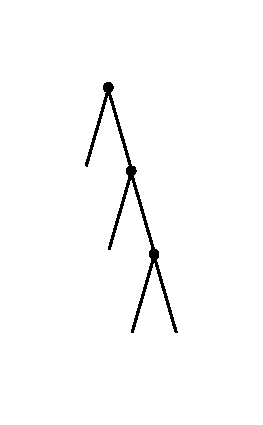
\includegraphics[scale=1]{figures/standard}
}
\caption[]{Three trees of various shapes but equal size.}
\label{figure:standard-representation}
\end{figure}

\subsection{\mono{normalize/1}}

\begin{verbatim}
normalize a = normalize-aux a 0 0

normalize-aux 0     0     an = an
normalize-aux 0     bl.br an = normalize-aux bl br    an
normalize-aux 0.ar  b     an = normalize-aux ar b     0.an
normalize-aux al.0  b     an = normalize-aux al b     0.an
normalize-aux al.ar b     an = normalize-aux ar al.b  0.an

\end{verbatim}

\subsubsection{Correctness}

\mono{normalize/1} makes use of an auxiliary procedure, \mono{normalize-aux/3},
for which we can provide the following argument descriptions:

\begin{enumerate}

\item The tree to be normalized.

\item An auxiliary tree.

\item A normalized tree.

\end{enumerate} 

The idea of the algorithm is to move right-wise down the tree to be normalized,
constructing an auxiliary tree containing all left-wise child nodes, if any.

The return value is the normalized tree, i.e. the third argument. Hence, we
must increase the size of the normalized tree each time we move right-wise down
the tree to be normalized.

Once we reach the right-most leaf of the tree to be normalized we return the
normalized tree if the auxiliary tree is empty. Otherwise, we normalize the
right child of the auxilary tree, with the left child of the auxiliary as the
new auxiliary tree, and the normalized tree constructed thus far as the initial
normalized tree.

\subsubsection{Time complexity}

Coming soon..

\subsubsection{Space complexity}

Coming soon..

\subsection{\mono{less/2}}\label{section:d-size-less}

We'll define the function \mono{normalize/1} further below to transform any
\D{} value into its standard representation. For now we'll assume that we have
such a function in scope and define \mono{less/2} for determining whether the
value of the first argument is strictly less than the value of the second
argument.

In order to define such a boolean-valued function we need a convention for
representing the boolean values $true$ and $false$ in \D{}. We'll adopt the
C-like convention:

\begin{definition}

A $false$ value is represented by a leaf tree. A $true$ value is represented by
a non-leaf tree, i.e. a node.

\end{definition}

We're now ready to define the function \mono{less/2}:

\begin{lstlisting}[label={listing:d-less},caption={A definition of the \mono{less/2} function.}]
less a b := normalized-less (normalize a) (normalize b)

normalized-less 0 b := b
normalized-less _ 0 := 0
normalized-less _.a _.b := normalized-less a b
\end{lstlisting}

\subsubsection{Correctness}

\begin{proof}

Given \referToDefinition{standard-representation}, and the assumption that
$\proc{Normalize}(A)$ computes the standard representation of $A$, we know the
following:

\begin{enumerate}

\item $\left|A\right|\equiv\left|\proc{Normalize}(A)\right|$.

\item We'll walk through all the nodes if we perform a recursive
right-child-walk starting at $A$.

\item The same holds for $B$.

\end{enumerate}

It is also easy to see from lines
\ref{normalized-less-init-start}:\ref{normalized-less-init-end} that
$\proc{NormalizedLess}$ stops as soon as we reach the ``bottom'' of either $A$
or $B$.

Given \referToDefinition{size}, $A<B$ iff it bottoms out before $B$, that is,
we reach an instance of the recursion where both $IsLeaf(A)$ and $IsNode(B)$
hold.  In all other cases $A\geq B$, the cases specifically are:

\begin{itemize}

\item $IsLeaf(A)$ and $IsLeaf(B)$, then $\left|A\right|\equiv \left|B\right|$.

\item $IsNode(A)$ and $IsLeaf(B)$, then $\left|A\right|>\left|B\right|$

\end{itemize}

Last but not least, due to all data values being finite, eventually one of the
trees does bottom out.

\end{proof}

\subsubsection{Time complexity}

Given that the binary trees $A$ and $B$ are in standard representation when we
enter the auxiliary procedure, $\proc{NormalizedLess}$, it is fairly easy to
get an upper bound on the running time of $\proc{NormalizedLess}$ itself.

Indeed, the running time of $\proc{NormalizedLess}$ itself is
$O\left(\proc{Max}\left(\left|A\right|,\left|B\right|\right)\right)$, since we
just walk down the trees until one of them bottoms out. 

We haven't yet defined the procedure $\proc{Normalize}$ yet. Hence, the only
thing that we can say about the running time of $\proc{Less}$ in general is
that it is $O\left(\proc{Normalize}(A) + \proc{Normalize}(B) +
\proc{Max}\left(\left|A\right|,\left|B\right|\right) \right)$.

\subsubsection{Space complexity}

Coming soon..

\section{Built-in high-order
functions}\label{section:language-higher-order-built-ins}

Although \mono{D} is initially a first-order language, we will ignore that
limitation for a bit and define a few higher-order functions to provide some
syntactical sugar to the language. Beyond the discussion in this section, these
higher-order functions should be regarded as \mono{D} built-ins.

\subsubsection{Branching}

In the following definition, the variable names \mono{true} and \mono{false}
refer to expressions to be executed in either case.

\begin{verbatim}
if 0 _ false := false
if _._ _ true := true
\end{verbatim}

As you can see, we employ the C convention that any value other than $0$ is a
``truthy'' value, and the expression \mono{true} is returned.

Although the call-by-value nature of the language does not allow for
short-circuiting the if-statements defined in such a way, this shouldn't be any
impediment to further analysis.

\subsection{Boolean operations}

\begin{verbatim}
and _._ _._ = 0.0
and _ _ = 0

or 0 0 = 0
or _ _ = 0.0
\end{verbatim}


\section{Sample programs}\label{section:d-samples}

As an illustration of the language syntax, take a look at the programs in
\referToListing{reverse}, \referToListing{fibonacci} and
\referToListing{ackermann}.

\begin{lstlisting}[label=listing:reverse,
  caption={A program that reverses the order of the nodes of some supplied tree.}]
reverse 0 := 0
reverse left.right := (reverse right).(reverse left)

reverse input
\end{lstlisting}

\begin{lstlisting}[label=listing:fibonacci,
  caption={A program that computes the $n^{th}$ fibonacci when supplied with some $n$.}] 
fibonacci n = fibonacci-aux (normalize n) 0 0

fibonacci-aux 0 x y := 0
fibonacci-aux 0.0 x y := y
fibonacci-aux 0.n x y := fibonacci-aux n y (add x y)

fibonacci input
\end{lstlisting}

\begin{lstlisting}[label=listing:ackermann,
  caption={The Ackermann-P\'eter function.}]
ackermann 0 n := 0.n
ackermann a.b 0 := ackermann (decrease a.b) 1
ackermann a.b c.d := ackermann (decrease a.b) (ackermann a.b (decrease c.d))

ackermann input input
\end{lstlisting}


\newcommand{\D}{$\Delta$}
\chapter{The language \D{}}

The goal of this work is to describe a few automated termination analysis
techniques, and in particular, size-change termination. In order to allow for
the following chapters to retain a modest level of abstraction to the Turing
machine, such that the techniques are described for an environment that is
modestly applicable to solving moderate programming problems, a Turing complete
language \D{} is introduced.

The intent of the language is hence two-fold, (1) aid the descriptions of the
automated termination analysis techniques in further chapters and (2) be
relatively modern in the subjective sense of expressiveness.

Expressiveness of a language depends on its initially intended domains. Of
course, Turing complete languages are known to be universally applicable,
however some languages are just more fine tuned to solving some problems, while
others are better tuned for solving other problems, hence the domain-specific
and subjective term of expressiveness.

\D{} is a language that disregards the aspect of abstract data structures.
Hence, many data driven programs \emph{will} be hard to write in \D{} due to,
for instance, the complete absence of types. This is of course, relative.
Various aspects of the data flow of a program can be important to various
automated termination analysis techniques, in particular size-change
termination. Hence, \D{} is not completely useless and does have data and even
simple ways of analyzing the sizes and shapes of its values and branching
depending on the outcome of such analyses.

\section{General properties}

One of the fundamental concepts required of the
language of application is that it's datatypes are well-founded. That is, any
subset $S$ of the range of values of some well-defined type has a value $s$
s.t. $\forall {s'\in S}\ s\leq s'$. This makes it ideal to chose some
oversimplistic data type structure rather than an army of basic types. Besides,
an apropriately defined basic data type should be able to represent arbitrarily
complex data values.

The language is initially first-order since the size-change termination
principle is first described for first-order programs later on in this work.
However, the language is designed so that it is easy to turn it into a
high-level language without much effort. This may prove necessary as we try to
expand size-change termination to higher-order programs.

The language is a call-by-value and purely functional to avoid any problems
that could arise from regarding lazy programs or where the notion of a global
state of the machine is relevant. Simply put, this is done to ensure elegance
of further proof with the help of the language.

The language \D{} is also Turing complete in the sense that it can model the
Turing machine.

\begin{frame}

\frametitle{\D{}, values and shapes}

\begin{columns}

\column{0.3\textwidth}
\begin{center}
$$b\in\mathbb{B}$$
\includegraphics[scale=0.5]{figures/value}
\end{center}

\column{0.3\textwidth}

\begin{center}
{\fontsize{40}{20}$\succ$}
\end{center}

\column{0.3\textwidth}

\begin{center}
$$s\in\mathbb{S}$$
\includegraphics[scale=0.5]{figures/shape}
\end{center}

\end{columns}

\end{frame}

\begin{frame}

\frametitle{\D{}, shapes and shapes}

\begin{columns}

\column{0.3\textwidth}
\begin{center}
$$s_1\in\mathbb{S}$$
\includegraphics[scale=0.5]{figures/shape}
\end{center}

\column{0.3\textwidth}

\begin{center}
{\fontsize{40}{20}$\succ$}
\end{center}

\column{0.3\textwidth}

\begin{center}
$$s_2\in\mathbb{S}$$
\includegraphics[scale=0.5]{figures/shape-2}
\end{center}

\end{columns}

\end{frame}

\begin{frame}

\frametitle{Disjoint shapes}

\begin{center}

$$s_1\cap s_2=\emptyset\quad\text{iff}\quad B_1\cap B_2=\emptyset$$

where

$$s_1,s_2\in\mathbb{S} \wedge B_1=\{b\mid b\in\mathbb{B} \wedge b\succ
s_1\}\wedge B_2=\{b\mid b\in\mathbb{B} \wedge b\succ s_2\}$$

\end{center}

\end{frame}

% TODO: All patterns now have a name.

\begin{frame}

\begin{center}

Given a shape $s_i\in\mathbb{S}$, we define the {\bf sibling set} $S^d_i$, to
be the pairwise disjoint set of shapes disjoint with $s_i$.

\end{center}

\end{frame}

\begin{frame}[fragile]

\begin{textblock}{1}(13.8,-3.5)$(35)$\end{textblock}

\begin{lstlisting}
data Pattern
  = PNil
  | PVariable String
  | PNode Pattern Pattern

getSiblings :: Pattern -> [Pattern]

getSiblings PNil =
  [PNode (PVariable "_") (PVariable "_")]

getSiblings (PVariable _) = []

getSiblings (PNode leftP rightP) =
  let
    leftS = getSiblings leftP
    rightS = getSiblings rightP
    leftInit = map (\s -> PNode leftP s) rightS
    rightInit = map (\s -> PNode s rightP) leftS
  in
    [PNil] ++
      leftInit ++ rightInit ++
      interleaveSiblings name leftS rightS
\end{lstlisting}

\end{frame}

\begin{frame}

\begin{align*}
T(1)&=4\\
T(n)&=1+T(n-1)+T(n-1)+T(n-1)\cdot T(n-1)
\end{align*}

\end{frame}

\section{Syntax}\label{section:d-syntax}

We describe the syntax of \D{} in terms of an extended Backus-Naur
form\footnote{The extension lends some constructs from regular expressions to
achieve a more concise dialect. The extension is described in detail in
\referToAppendix{ebnf}.}. This is a core syntax definition, and other, more
practical, syntactical features may be defined later on as needed. The initial
non-terminal is $\nonterm{program}$.

\begin{align}
\nonterm{program}\ ::=&\ \nonterm{clause}^*\ \nonterm{expression}\\
\nonterm{expression}\ ::=&\ \nonterm{element}\ (\ \term{.}\ \nonterm{expression}
\ )\ ?\\
\nonterm{element}\ ::=&\ \term{0}\ |\ \term{(}\ \nonterm{element}\ \term{)}\ |
\ \nonterm{name}\ |\ \nonterm{application}\\
\nonterm{application}\ ::=&\ \nonterm{name}
\ \nonterm{expression}^+\\
\nonterm{clause}\ ::=&\ \nonterm{name}\ \nonterm{pattern}^+
\ \term{:=}\ \nonterm{expression}\\
\label{nonterm-pattern}
\nonterm{pattern}\ ::=&\ \nonterm{pattern-element}\ (\ \term{.}
\ \nonterm{pattern}\ )\ ?\\
\label{nonterm-pattern-element}
\nonterm{pattern-element}\ ::=&\ \term{0}\ |\ \term{\_}\ |\ \term{(}
\ \nonterm{pattern}\ \term{)}\ |\ \nonterm{name}\\
\nonterm{name}\ ::=&\ [\term{a}\mathmono{-}\term{z}]
\ \left (\ [\term{-}\ \term{a}\mathmono{-}\term{z}]^*
\ [\term{a}\mathmono{-}\term{z}]\ \right )?
\end{align}

\begin{definition} \referToTable{sos-definitions} defines shorthands for
various language constructs. We'll often refer to these in further discussions.
Additionally, we'll let the atoms $0$ and $\_$ represent
themselves.\end{definition} 

\makeTable[h!]
{sos-definitions}
{Shorthands for various language constructs for use in latter discussions. We
provide shorthands for an instance, a list, and the space of a construct. For
instance, $x$ is some particular expression, $X$ is some particular list of
expressions, and $\mathbb{X}$ is the set of all possible expressions.}
{|l|c|c|c|}
{\textbf{Description}&\textbf{Instance}&\textbf{Finite list}&\textbf{Space}}
{
Expression & $x$ & $X$ & $\mathbb{X}$\\
Element (of an expression) & $e$ & $E$ & $\mathbb{E}$\\
Function & $f$ & $F$ & $\mathbb{F}$\\
Clause & $c$ & $C$ & $\mathbb{C}$\\
Pattern & $p$ & $P$ & $\mathbb{P}$\\
Value & $b$ & $B$ & $\mathbb{B}$\\
Name & $v$ & $V$ & $\mathbb{V}$\\
Program & $r$ & $R$ & $\mathbb{R}$
}

%\begin{definition} The \nonterm{expression} at the end of \nonterm{program} can
%be considered as the main clause of a program, which we'll refer to as
%$c_{main}$.\end{definition}

\begin{definition} For any given $v\in\mathbb{V}$ and $P\subset\mathbb{P}$,
we say that $v\in P$ if $v$ occurs in some $p\in P$.\end{definition}

\begin{definition}\label{definition:clause-tuple} A clause $c\in\mathbb{C}$ is
a tuple $\left\langle v,P,x \right\rangle$, where $v\in\mathbb{V}$ is the name
of the clause, $P\subset\mathbb{P}$ is a non-empty list of patterns of the
clause, and $x\in\mathbb{X}$ is the expression of the clause. $P$ is ordered by
occurrence of the patterns in the program text.\end{definition}

\begin{definition} We say that a clause $c= \left\langle v,P,x \right\rangle$
``accepts'' an argument list $B$ iff $|P|=|B|$ and $\forall\ \{i\mid 0\geq i <
|P|\}\ b_i\in B \wedge p_i\in P \wedge b_i\succ p_i$.\end{definition}

\begin{definition}\label{definition:function-tuple} A function $f\in\mathbb{F}$
is a tuple $\left\langle v,C \right\rangle$, where $v \in \mathbb{V}$ is the
name of the function, and $C\subset\mathbb{C}$ is the non-empty list of clauses
of the function. It must hold for $C$ that $\forall\ c\in C\
\left(c=\left\langle v_c, P_c, x_c \right\rangle \wedge v_c=v\right)$ and
$\forall\ c_1,c_2\in C\ \left(c_1=\left\langle v_1, P_1, x_1 \right\rangle
\wedge c_2=\left\langle v_2, P_2, x_2 \right\rangle \wedge |P_1|=|P_2|\right)$.
$C$ is ordered by occurrence of the clauses in the program
text.\end{definition}

\begin{definition} A signature of some function $f=\left\langle v, C
\right\rangle$ is the tuple $\left\langle v,|P| \right\rangle$, s.t.
$\forall\ c\in C_f\ |P_c|=|P|$. We'll adopt the Erlang notation when talking
about function signatures, i.e. if we have a function \mono{less} that takes in
two parameters, we'll refer to it as \mono{less/2}.\end{definition}

We assume for it to be fairly simple to construct the set $F$ of a given
program $r$ given the set of clauses $C$ derived during syntactic analysis of
the program text.

\begin{definition} A program $r$ is a tuple $\left\langle F,x \right\rangle$,
where $F\subset\mathbb{F}$ is the list of functions defined in program $r$, and
$x$ is the expression of program $r$.\end{definition}

\begin{definition}\label{definition:function-call} A function call is a tuple
$\left\langle v, X \right\rangle$, where $v\in\mathbb{V}$ is the name of the
callee, and $X\subset\mathbb{X}$ is a non-empty list of arguments for the
function call, ordered by occurrence of the expressions in the program
text.\end{definition}

0-ary clauses are disallowed to avoid having to deal with constants in general.
The term $\term{\_}$ in $\nonterm{pattern-element}$ is the conventional
wildcard operator; it indicates a value that won't used in the clause
expression, but some value has to be there for an argument to match the
pattern. Furthermore, as will be clear from the semantics, multiple occurrences
of \term{\_} in a clause pattern list does not indicate that the same value has
to be in place for each \term{\_}. 

\begin{definition} When describing various values and patterns in definitions,
theorems, proofs, etc. we'll sometimes make use of $\_$ to denote parts of the
value or pattern that are irrelevant to the said definition, theorem, proof,
etc.\end{definition}

% TODO this should be clear from the semantics.

% Multiple wildcards in the parameter list indicate possibly different value
% arguments, while multiple occurances of the same variable name in the parameter
% list are disallowed.

\subsection{Patterns constitute shapes}

The nonterminal declarations for patterns, in particular \ref{nonterm-pattern}
and \ref{nonterm-pattern-element}, indicate that a pattern are equatable to
shapes.

\begin{definition}\label{definition:pattern-corresponds-shape} The pattern
\term{0} corresponds to the leaf shape. The patterns \term{\_} and
\nonterm{name} correspond to triangle shapes. Any pattern \mono{a.b}
corresponds to the shape $a\cdot b$ iff the pattern \mono{a} corresponds to the
shape $a$ and the pattern \mono{b} corresponds to the shape
$b$.\end{definition}

\begin{definition}\label{definition:pattern-is-shape} $\forall\ p\in\mathbb{P}\
\forall\ s\in\mathbb{S}\ p=s$ iff $p$ corresponds to $s$ as by
\referToDefinition{pattern-corresponds-shape}.\end{definition}

\begin{definition} We overload the binary relation $\succ$ with the set\\
$\left\{ \left\langle p_1,p_2 \right\rangle\mid p_1,p_2\in\mathbb{P},
s_1,s_2\in\mathbb{S} \wedge p_1=s_1 \wedge p_2=s_2
\right\}$.\end{definition}

\subsection{Unary functions from multivariate functions}

The patterns of a clause as well as the arguments of a function call get
special treatment in \D{} in that they according to
\referToDefinition{clause-tuple} and \referToDefinition{function-call} are
ordered by their occurrence in the program text. This order is important to
make sure that the appropriate argument is matched against the appropriate
pattern. 

While this is setup is practical for the programmer, it is of no use to us due
to \referToTheorem{multivariate-to-unary}. In latter discussions, this
particular theorem allows us to keep to unary functions, and regard the
extension to multivariate functions as a fairly simple matter.

\begin{theorem}\label{theorem:multivariate-to-unary} Any multivariate function
in \D{} can be represented with a unary function.\end{theorem}

\begin{proof}

Given a multivariate function $f= \left\langle v,C \right\rangle$:

\begin{enumerate}

\item For each clause $c\in C$, where $c=\left\langle v,P,x \right\rangle$,
replace the pattern list $P$ with $P'=\{p\}$. Construct $p$ by initially
letting $p=0$, and folding left-wise over $P$, performing $p=p\cdot p'$ for
each $p'\in P$. 

\item For each call $\left\langle v, X\right\rangle$ to function $f$, replace
$X$ with the set $X'=\{x\}$, where $x$ has been constructed in a manner
equivalent to the pattern $p$ above.

\end{enumerate}

It is easy to see that both the constructed patterns and expressions are indeed
valid patterns and expressions, and that $f$ hence becomes a unary
function.\end{proof}

As this transformation is relatively simple to perform, we redefine the generic
clause tuple to have but one pattern in place of a list. 

\begin{definition}\label{definition:unary-clause} We redefine the clause $c$ to
be the tuple $\left\langle v,p,x\right\rangle$, where $v\in\mathbb{V}$ is the
name of the clause, $p\in\mathbb{P}$ is the pattern of the clause, and
$x\in\mathbb{X}$ is the expression of the clause.\end{definition}

\begin{definition}\label{definition:unary-function-call} We redefine a function
call to be the tuple $\left\langle v,x\right\rangle$, where $v\in\mathbb{V}$ is
the name of the callee, and $x\in\mathbb{X}$ is the argument to the (always
unary) callee.\end{definition}

\section{Semantics}\label{section:d-sos}

Revise the context of an expression within a function call, it should always be
the context upon entering the function call! Or even better, the context when
the function was defined!


\textbf{Perhaps pattern matching must be exhaustive in general.}

\textbf{Every subsequent definition must be strictly less specific than the former.}




In the following section we describe the semantics of \D{} using structured
operational semantics. The syntax used to define the reduction rules is largely
equivalent to the Aarhus report\cite{sos}, but differs slightly\footnote{The
syntax applied here is described in further detail in \referToAppendix{sos}.}.
The most notable about the syntax used here is the following:

\begin{itemize}

\item Rules should be read in increasing order of equation number.

\item If some rule with a lower equation number makes use of an undefined
reduction rule, it is because the reduction rule is defined under some higher
equation number.

\item Rules can be defined in terms of themselves, i.e. they can be recursive,
even mutually recursive.

\end{itemize}

The syntax aside, \referToTable{sos-definitions} defines a few lower-letter
shorthands for various constructs. Additionally, we'll let the capital
equivalents of these letters represent a sets of the respective construct, as
well as let the atoms $0$ and $\_$ represent themselves in the reduction rules.
It is also worth noting that $\forall\ v\in V\ :\ v\in \mathbb{B}$.

\makeTable[h!]
{sos-definitions}
{Overview of some of the shorthands used in this text. The column \textbf{A}
refers to all possible instances of the given construct, i.e.  $\mathbb{B}$
reffers to all constructable values in \D{}. The column \textbf{P} refers to
all the instances of the given construct in a given program, i.e. $N$ reffers
to all the names in a given program. The column \textbf{I} reffers to specific
instances of the given constructs, i.e. $x$ reffers to a particular
expression.}
{|l|c|c|c|}
{\textbf{Description}&\textbf{I}&\textbf{P}&\textbf{A}}
{
Expression & $x$ & $X$ & $\mathbb{X}$\\
Element (of an expression) & $e$ & $E$ & $\mathbb{E}$\\
Pattern & $p$ & $P$ & $\mathbb{P}$\\
Value(binary tree) & $b$ & $B$ & $\mathbb{B}$\\
Name & $n$ & $N$ & $\mathbb{N}$
}

\subsection{The memory model}\label{section:d-semantics-memory}

Memory is considered in terms of a set of value stacks, $\sigma$. Every stack
has a unique identifier $n\in N$, that is, each variable in a given program
gets a value stack. As we enter a new scope, we bind a variable to a value,
that is, we push that value on top of the corresponding stack. We pop the value
off the corresponding stack as we leave the scope at the entry to which the
variable was bound.

An expression at a certain scope depth only has access to variables at the same
scope depth. This is to ensure static scope. We won't adhere to this problem
explicitly in the semantics, but instead ask you to simply keep it in mind.

\subsubsection{Functions and variables}

Due to \D{} being a first-order language, we should make sure to separate the
function and variable spaces. We'll represent these by $\phi$ and $\gamma$,
respectively.

Whenever we use $\sigma$, $\phi$ or $\gamma$ in set notation, we imply the sets
of the names of functions and variables, and not the stacks themselves
corresponding to those names.  Hence, $\sigma=\phi\cup\gamma$, and to keep \D{}
first-order we add the limitation that $\phi\cap\gamma=\emptyset$.

\subsubsection{Making \D{} higher order}

The only change that this would require is to let $\phi=\gamma=\sigma$.

\subsection{Declaration}

A declaration with a name $n$, a \emph{non-empty} pattern
list $[p]$ and an expression $e$ is stored in the function space $\phi$:

\begin{equation}\label{sem:declaration}
{\displaystyle
  \left\langle \phi(n)\leftarrow \left\langle P, x\right\rangle\right\rangle
  \Rightarrow
  \phi'
\over\displaystyle
  \left\langle n, P, x, \phi\right\rangle
  \Rightarrow
  \phi'
}
\end{equation}

\subsection{Expression evaluation}

An expression $x$ is either the element $e$, or a construction of an element
$e'$ with another expression $x'$. That is, the binary infix operator $\cdot$
is right-associative, and has the following operational semantics:

\everymath{\displaystyle}

\begin{equation}
{\displaystyle
  \left\langle \proc{Single}, x,\sigma\right\rangle
  \rightarrow
  \left\langle v,\sigma\right\rangle
\vee
  \left\langle \proc{Chain}, x,\sigma\right\rangle
  \rightarrow
  \left\langle v,\sigma\right\rangle
\over\displaystyle
  \left\langle x,\sigma\right\rangle
  \rightarrow
  \left\langle v,\sigma\right\rangle
}
\end{equation}

\begin{equation}
{\displaystyle
  x\rightarrow e
\wedge
  \left\langle e,\sigma\right\rangle
  \rightarrow
  \left\langle v,\sigma\right\rangle
\over\displaystyle
  \left\langle \proc{Single}, x,\sigma\right\rangle
  \rightarrow
  \left\langle v,\sigma\right\rangle
}
\end{equation}

\begin{equation}
{\displaystyle
  x\Rightarrow e_1\cdot x_1
\wedge
  \left\langle e_1,\sigma\right\rangle
  \rightarrow
  \left\langle v_1,\sigma\right\rangle
\wedge
  \left\langle x_1,\sigma\right\rangle
  \rightarrow
  \left\langle v_2,\sigma\right\rangle
\over\displaystyle
  \left\langle \proc{Chain}, x, \sigma\right\rangle
  \rightarrow
  \left\langle v, \sigma\right\rangle
}
\quad(\text{where }v_1\cdot v_2=v)
\end{equation}

\subsection{Element evaluation}

According to the syntax specification, an element of an expression can either
be the atom $0$, or an application. We'd like to distinguish between variables
and functions, and we do that  

\begin{equation}
{\displaystyle
\left(
    e\Rightarrow 0
  \wedge
    v\equiv 0
\right)
\vee
{\displaystyle
    e\Rightarrow n
\over\displaystyle
    \beta(n)\Rightarrow v
}
\vee
{\displaystyle
    e\Rightarrow \left\langle n, X\right\rangle
\over\displaystyle
    \left\langle n,X,\sigma\right\rangle
    \Rightarrow
    \left\langle v,\sigma\right\rangle
}
\over\displaystyle
\left\langle e,\sigma\right\rangle
\Rightarrow
\left\langle v,\sigma\right\rangle
}
\end{equation}

\subsection{Function application}

\begin{equation}
{\displaystyle
{\displaystyle
{\displaystyle
  \left\langle n, \phi\right\rangle
  \Rightarrow
  \left\langle P, x, \phi\right\rangle
\over\displaystyle
  \left\langle P, X, \sigma\right\rangle
  \Rightarrow
  \sigma'
}
\over\displaystyle
  \left\langle x, \sigma'\right\rangle
  \Rightarrow
  \left\langle v,\sigma'\right\rangle
}
\over\displaystyle
    \left\langle n,X,\sigma\right\rangle
    \Rightarrow
    \left\langle v,\sigma\right\rangle
}
\end{equation}

\subsection{Pattern matching}

\begin{equation}
{\displaystyle
{\displaystyle
  \left\langle P_{head}, X_{head}, \sigma\right\rangle
  \Rightarrow
  \sigma''
\over\displaystyle
  \left\langle P_{tail}, X_{tail}, \sigma''\right\rangle
  \Rightarrow
  \sigma'
}
\over\displaystyle
  \left\langle P, X, \sigma\right\rangle
  \Rightarrow
  \sigma'
}
\end{equation}

\begin{equation}
{
  \left\langle\proc{I}, p,x,\sigma\right\rangle
  \Rightarrow
  \left\langle p',x',\sigma'\right\rangle
\vee
  \left\langle\proc{Z}, p,x,\sigma\right\rangle
  \Rightarrow
  \left\langle p',x',\sigma'\right\rangle
\vee
  \left\langle\proc{N}, p,x,\sigma\right\rangle
  \Rightarrow
  \left\langle p',x',\sigma'\right\rangle
\vee
  \left\langle\proc{P}, p,x,\sigma\right\rangle
  \Rightarrow
  \left\langle p',x',\sigma'\right\rangle
}\over{
  \left\langle p, x, \sigma\right\rangle
  \Rightarrow
  \left\langle p', x', \sigma'\right\rangle
}
\end{equation}

For the sake of an elegant notation, we'll override the function $\cdot$ for
patterns.

\begin{definition}

A pattern is an unlabeled of binary tree which is either empty or consists of
an unlabeled node with a $0$, $\_$, name, or a pattern as it's left and right
child. 

\end{definition}

\begin{definition}

Let the set of all possible patterns be denoted by $\mathbb{P}$.

\end{definition}

\begin{definition}

The function $\cdot
:\mathbb{P}\times\mathbb{P}\rightarrow\mathbb{P}$ constructs a pattern node with the
two arguments as it's left and right child, respectively. 

\end{definition}

\begin{equation}
{
    p\Rightarrow \_\cdot p'
  \wedge
    x\Rightarrow e\cdot x'
  \wedge
    \sigma\Rightarrow\sigma'
}\over{
  \left\langle\proc{Underscore}, p,x,\sigma\right\rangle
  \Rightarrow
  \left\langle p',x',\sigma'\right\rangle
}
\end{equation}

\begin{equation}
{
    p\Rightarrow 0\cdot p'
  \wedge
    x\Rightarrow e\cdot x'
  \wedge
    \sigma\Rightarrow\sigma'
}\over{
  \left\langle\proc{Zero}, p,x,\sigma\right\rangle
  \Rightarrow
  \left\langle p',x',\sigma'\right\rangle
}
\end{equation}


\begin{equation}
{\displaystyle
{\displaystyle
{\displaystyle
    p\Rightarrow n\cdot p'
  \wedge
    x\Rightarrow e\cdot x'
\over\displaystyle
    \left\langle e,\sigma\right\rangle
    \Rightarrow
    \left\langle v,\sigma\right\rangle
}\over\displaystyle
    \left\langle\sigma(n)\leftarrow v\right\rangle
    \Rightarrow
    \sigma'
}\over\displaystyle
  \left\langle\proc{Name}, p,x,\sigma\right\rangle
  \Rightarrow
  \left\langle p',x',\sigma'\right\rangle
}
\end{equation}

\begin{equation}
{\displaystyle
{\displaystyle
    p\Rightarrow p''\cdot p'  
  \wedge
    x\Rightarrow x''\cdot x'
\over\displaystyle
  \left\langle p'', x'', \sigma\right\rangle
  \Rightarrow
  \sigma'
}
\over\displaystyle
  \left\langle\proc{Pattern}, p,x,\sigma\right\rangle
  \Rightarrow
  \left\langle p',x',\sigma'\right\rangle
}
\end{equation}

\input{language/input}
\section{Size}

For the purposes of talking about size-change termination, we also need to
define the notion of size, and be sure to do so in such a way so that all
possible data values are well-founded.

\begin{definition}\label{definition:size}

Size of a value in \D{} is the number of nodes in the tree representing
that value.

\end{definition}

The ``well-foundedness'' of \D{}'s data values, given such a definition can be
argued for by proving a bijective relation between $\mathbb{B}$ and
$\mathbb{N}$. This would imply that we can define the relation $<$ on \D{}'s
data values, which we know to be well-founded.

We start by formally proving that \referToDefinition{size} yields a many-to-one
mapping of \D{}'s data values to the natural numbers.

First, we prove, by induction, that any natural number can be represented in
\D{}:

\begin{proof}\ \\

\begin{description}[\setleftmargin{70pt}\setlabelstyle{\bf}]

\item [Base] The atom $0$ has no nodes, and hence represents the value $0$.

\item [Assumption] If we can represent the $n\in\mathbb{N}$ in \D{}, then
we can also represent the number $n+1\in\mathbb{N}$. 

\item [Induction] Let $n$ be represented by some binary tree $A$, then $n+1$
can be represented by $0\cdot A$. 

\end{description}

\end{proof}

Second, we prove, also by induction, that any value in \D{} has one and only
one representation in $\mathbb{N}$.

\begin{proof}\ \\

\begin{description}[\setleftmargin{70pt}\setlabelstyle{\bf}]

\item [Base] The atom $0$ has no nodes, and hence corresponds only to the value
$0$.

\item [Assumption]

\begin{enumerate}

\item If the binary tree $A$ has only one representation $n\in\mathbb{N}$, then
$\left|0\cdot A\right|\equiv n+1$ and $\left|A\cdot 0\right|\equiv n+1$.

\item If the binary tree $A$ has only one representation $n\in\mathbb{N}$, and
the binary tree $B$ has only one representation $m\in\mathbb{N}$, then
$\left|A\cdot B\right|\equiv n+m+1$ and $\left|B\cdot A\right|\equiv n+m+1$.

\end{enumerate}

\item [Induction]

By definition of the binary function $\cdot$, any given node $A$ with left
child $A_{left}$ and right child $A_{right}$ has the size:

$$\left|A\right|=1+\left|A_{left}\right|+\left|A_{right}\right|$$

Hence, any value in \D{} must have one and only one representation in
$\mathbb{N}$.

\end{description}

\end{proof}

\referToDefinition{size} \emph{almost} allows us to devise an algorithm to
compare the sizes of data values. The problem withstanding is that two
different values can have rather diverging tree representations. Hence,
comparing them, using only the operations defined in \referToSection{d-sos}, is
seemingly impossible unless we initially, or along the way, transform the
binary trees being compared into some sort of a \emph{standard representation}.
We'll define this representation, recursively, as follows:

\begin{definition}\label{definition:standard-representation}

A binary tree in standard representation is a binary tree that either is a leaf
or a node having a leaf as its left child and a binary tree in standard
representation as its right child.

\end{definition}

Intuitively, a binary tree in standard representation is just a tree that only
descends along the right side. Comparing the sizes of two trees in this
representation is just a matter of walking the descending in the two trees
simultaneously, until one of them, or both, bottom out. If there is a tree that
bottoms out strictly before another, that is the lesser tree by
\referToDefinition{size}. \referToFigure{standard-representation} showcases
some examples.

\begin{figure}[htbp!]
\centering
\subfigure[{Not in standard representation}]
{
  \includegraphics[scale=1]{figures/first-non-standard}
}
\subfigure[{Not in standard representation}]
{
  \includegraphics[scale=1]{figures/second-non-standard}
}
\subfigure[{Standard representation}]
{
  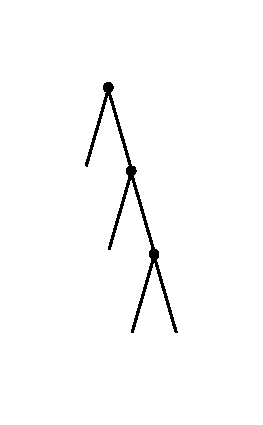
\includegraphics[scale=1]{figures/standard}
}
\caption[]{Three trees of various shapes but equal size.}
\label{figure:standard-representation}
\end{figure}

\subsection{\mono{normalize/1}}

\begin{verbatim}
normalize a = normalize-aux a 0 0

normalize-aux 0     0     an = an
normalize-aux 0     bl.br an = normalize-aux bl br    an
normalize-aux 0.ar  b     an = normalize-aux ar b     0.an
normalize-aux al.0  b     an = normalize-aux al b     0.an
normalize-aux al.ar b     an = normalize-aux ar al.b  0.an

\end{verbatim}

\subsubsection{Correctness}

\mono{normalize/1} makes use of an auxiliary procedure, \mono{normalize-aux/3},
for which we can provide the following argument descriptions:

\begin{enumerate}

\item The tree to be normalized.

\item An auxiliary tree.

\item A normalized tree.

\end{enumerate} 

The idea of the algorithm is to move right-wise down the tree to be normalized,
constructing an auxiliary tree containing all left-wise child nodes, if any.

The return value is the normalized tree, i.e. the third argument. Hence, we
must increase the size of the normalized tree each time we move right-wise down
the tree to be normalized.

Once we reach the right-most leaf of the tree to be normalized we return the
normalized tree if the auxiliary tree is empty. Otherwise, we normalize the
right child of the auxilary tree, with the left child of the auxiliary as the
new auxiliary tree, and the normalized tree constructed thus far as the initial
normalized tree.

\subsubsection{Time complexity}

Coming soon..

\subsubsection{Space complexity}

Coming soon..

\subsection{\mono{less/2}}\label{section:d-size-less}

We'll define the function \mono{normalize/1} further below to transform any
\D{} value into its standard representation. For now we'll assume that we have
such a function in scope and define \mono{less/2} for determining whether the
value of the first argument is strictly less than the value of the second
argument.

In order to define such a boolean-valued function we need a convention for
representing the boolean values $true$ and $false$ in \D{}. We'll adopt the
C-like convention:

\begin{definition}

A $false$ value is represented by a leaf tree. A $true$ value is represented by
a non-leaf tree, i.e. a node.

\end{definition}

We're now ready to define the function \mono{less/2}:

\begin{lstlisting}[label={listing:d-less},caption={A definition of the \mono{less/2} function.}]
less a b := normalized-less (normalize a) (normalize b)

normalized-less 0 b := b
normalized-less _ 0 := 0
normalized-less _.a _.b := normalized-less a b
\end{lstlisting}

\subsubsection{Correctness}

\begin{proof}

Given \referToDefinition{standard-representation}, and the assumption that
$\proc{Normalize}(A)$ computes the standard representation of $A$, we know the
following:

\begin{enumerate}

\item $\left|A\right|\equiv\left|\proc{Normalize}(A)\right|$.

\item We'll walk through all the nodes if we perform a recursive
right-child-walk starting at $A$.

\item The same holds for $B$.

\end{enumerate}

It is also easy to see from lines
\ref{normalized-less-init-start}:\ref{normalized-less-init-end} that
$\proc{NormalizedLess}$ stops as soon as we reach the ``bottom'' of either $A$
or $B$.

Given \referToDefinition{size}, $A<B$ iff it bottoms out before $B$, that is,
we reach an instance of the recursion where both $IsLeaf(A)$ and $IsNode(B)$
hold.  In all other cases $A\geq B$, the cases specifically are:

\begin{itemize}

\item $IsLeaf(A)$ and $IsLeaf(B)$, then $\left|A\right|\equiv \left|B\right|$.

\item $IsNode(A)$ and $IsLeaf(B)$, then $\left|A\right|>\left|B\right|$

\end{itemize}

Last but not least, due to all data values being finite, eventually one of the
trees does bottom out.

\end{proof}

\subsubsection{Time complexity}

Given that the binary trees $A$ and $B$ are in standard representation when we
enter the auxiliary procedure, $\proc{NormalizedLess}$, it is fairly easy to
get an upper bound on the running time of $\proc{NormalizedLess}$ itself.

Indeed, the running time of $\proc{NormalizedLess}$ itself is
$O\left(\proc{Max}\left(\left|A\right|,\left|B\right|\right)\right)$, since we
just walk down the trees until one of them bottoms out. 

We haven't yet defined the procedure $\proc{Normalize}$ yet. Hence, the only
thing that we can say about the running time of $\proc{Less}$ in general is
that it is $O\left(\proc{Normalize}(A) + \proc{Normalize}(B) +
\proc{Max}\left(\left|A\right|,\left|B\right|\right) \right)$.

\subsubsection{Space complexity}

Coming soon..

\section{Built-in high-order
functions}\label{section:language-higher-order-built-ins}

Although \mono{D} is initially a first-order language, we will ignore that
limitation for a bit and define a few higher-order functions to provide some
syntactical sugar to the language. Beyond the discussion in this section, these
higher-order functions should be regarded as \mono{D} built-ins.

\subsubsection{Branching}

In the following definition, the variable names \mono{true} and \mono{false}
refer to expressions to be executed in either case.

\begin{verbatim}
if 0 _ false := false
if _._ _ true := true
\end{verbatim}

As you can see, we employ the C convention that any value other than $0$ is a
``truthy'' value, and the expression \mono{true} is returned.

Although the call-by-value nature of the language does not allow for
short-circuiting the if-statements defined in such a way, this shouldn't be any
impediment to further analysis.

\subsection{Boolean operations}

\begin{verbatim}
and _._ _._ = 0.0
and _ _ = 0

or 0 0 = 0
or _ _ = 0.0
\end{verbatim}


\section{Sample programs}\label{section:d-samples}

As an illustration of the language syntax, take a look at the programs in
\referToListing{reverse}, \referToListing{fibonacci} and
\referToListing{ackermann}.

\begin{lstlisting}[label=listing:reverse,
  caption={A program that reverses the order of the nodes of some supplied tree.}]
reverse 0 := 0
reverse left.right := (reverse right).(reverse left)

reverse input
\end{lstlisting}

\begin{lstlisting}[label=listing:fibonacci,
  caption={A program that computes the $n^{th}$ fibonacci when supplied with some $n$.}] 
fibonacci n = fibonacci-aux (normalize n) 0 0

fibonacci-aux 0 x y := 0
fibonacci-aux 0.0 x y := y
fibonacci-aux 0.n x y := fibonacci-aux n y (add x y)

fibonacci input
\end{lstlisting}

\begin{lstlisting}[label=listing:ackermann,
  caption={The Ackermann-P\'eter function.}]
ackermann 0 n := 0.n
ackermann a.b 0 := ackermann (decrease a.b) 1
ackermann a.b c.d := ackermann (decrease a.b) (ackermann a.b (decrease c.d))

ackermann input input
\end{lstlisting}


\chapter{Shape-Change Termination}

Size-change termination, despite being simple is powerful enough to determine
the halting property for a large class of programs. Many authors have extended
the principle to even wider classes of programs, e.g. extending it to handle
initially not well-founded data types \cite{bound-analysis}, applying it in
imperative programming languages \cite{heaps}, etc. 

One trouble with size-change termination as described in the previous chapter
is \referToLemma{cycle-reduce}. This lemma makes size-change termination weak
in the sense that the overall shape changes in a given call cycle are
\emph{not} considered, and instead, call cycles are constrained to
monotonically decreasing call cycles.  However, there may be programs that have
calls, or even call cycles, that in terms of size, increase a value for a
finite amount of time, until some condition is met, or as in the case of \D{},
a value has some particular shape.

Consider the program in \referToListing{size-change-fail} as an example of a
program for which regular size-change termination is unable to determine the
halting property, while the property itself would seem fairly simple to deduce.
This is a sample program where some value is increased in terms of size in a
call cycle, but only until the value matches a certain shape, the shape
required by a terminal clause.

\begin{lstlisting}[
  label=listing:size-change-fail,
  caption={A terminating program with a call cycle where a value is
  temporarily increased.}]
$f_0$: f a.b.c.d := a
$f_1$: f a := f a.0
f input
\end{lstlisting}

The extension proposed in this chapter is to be able to determine the halting
property for such a class of programs without reducing size of the class of
programs for which size-change termination can already deduce the halting
property.

In the discussion below we continue the assumptions from
\referToSection{size-change-termination}. In particular, all clauses in a
program are unary and bind at most one variable. Also, we can safely disregard
terminal clauses in call graphs.

\section{The class of programs considered}

Before we can speak of extending size-change termination to determine the
halting property for programs in the same class as
\referToListing{size-change-fail}, we need to formally define that class.

Actual conditions in \D{} can only be expressed in terms of patterns in
function clauses. Hence, we disregard programs that rely on equality or size
comparison conditions for termination, since this type of programs will often
already be covered by regular size-change termination, and if not, they at the
very least come down to recursive pattern matching.

As an example of a program where size-change termination is already prevalent,
consider a program that finds the $n^{th}$ Fibonacci number as the one already
presented in \referToSection{d-samples}. The function \mono{fibonacci-aux}
seemingly increases a value until a condition is met, in particular, until we
count one of the arguments down to \mono{0}. However, due to the fact that we
count that we decrease the value of that argument in \emph{recursive} clause of
the \mono{fibonacci-aux} functions, the halting property is certainly already
deducible by regular size-change termination.

Instead, we turn our attention to simpler programs, ones that rely solely on
conditions defined in terms of patterns. Consider again the program in
\referToListing{size-change-fail}. The function \mono{f} has only one terminal
clause, the one that accepts a shape as in \referToFigure{size-change-fail-f0}.
If the function argument has any other shape, i.e. either a shape as in
\referToFigure{size-change-fail-f1-0}, \referToFigure{size-change-fail-f1-1} or
\referToFigure{size-change-fail-f1-2}, then the recursive clause $f_1$ is
chosen. For any argument $b\in\mathbb{B}$, the clause $f_1$ replaces the
right-most child of the value, which is always \mono{0}, with a node.

For instance, the smallest possible argument $b\in\mathbb{B}$ is \mono{0}.  If
passed such a value, $f_1$ transforms it into a value that has a shape that
corresponds to \referToFigure{size-change-fail-f1-1}, which in turn transforms
the value into one that matches \referToFigure{size-change-fail-f1-2}, which in
turn transforms the value into one that matches
\referToFigure{size-change-fail-f0}, i.e. the terminal clause. What's more,
there are infinitely many other values that will match the shape
\referToFigure{size-change-fail-f1-1}, and for each of them, the clause $f_1$
will transform them into values that match
\referToFigure{size-change-fail-f1-2}, which will transform them into values
that match \referToFigure{size-change-fail-f0}.

\includeFigure{size-change-fail-f0}{The shape that the clause $f_0$ in
\referToListing{size-change-fail} will accept.}

\begin{figure}[htbp!]
\begin{minipage}{0.3\linewidth}
\centering
\includegraphics{figures/size-change-fail-f1-0}
\caption[]{The pattern \mono{0}.}
\label{figure:size-change-fail-f1-0}
\end{minipage}
\begin{minipage}{0.3\linewidth}
\centering
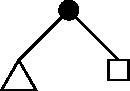
\includegraphics{figures/size-change-fail-f1-1}
\caption[]{The pattern \mono{a.0}.}
\label{figure:size-change-fail-f1-1}
\end{minipage}
\begin{minipage}{0.3\linewidth}
\centering
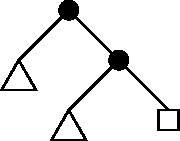
\includegraphics{figures/size-change-fail-f1-2}
\caption[]{The pattern \mono{a.b.0}.}
\label{figure:size-change-fail-f1-2}
\end{minipage}
\end{figure}

We shall henceforth say that a clause such as $f_1$ changes the shape of any
argument $b$ to \emph{eventually} match the shape corresponding to a pattern of
the terminal clause $f_0$. The task then becomes to determine for each call
cycle in a program whether it changes the shape of the argument to eventually
match some terminal clause.

\section{Preliminaries}

Before we continue with this extension we can make a few important observations
based on the semantics of function clauses in \D{}.

\subsection{Deducing leafs}\label{section:extend-deducing-zero}

The \mono{.} operator in the patterns of function clauses in \D{} is
right-associative. Hence, a pattern of the form \mono{a.b.c.d} is the same as
\mono{a.(b.(c.d))}. This implies that we can always construct a parenthesized
version of any valid pattern, indeed this is required to keep the syntax
unambiguous. This associativity can be overridden by the conventional use of
parentheses, e.g. a pattern like \mono{(a.b).c.d} is the same as
\mono{(a.b).(c.d)}. 

Consider the function defined in \referToListing{deducing-zero}. If $f_0$ and
$f_1$ both fail to accept some argument $b\in\mathbb{B}$, then $b$ must match
the pattern $0\cdot b'$, where $b'\geq 0$, that is, on entry to $f_2$, \mono{d}
is \emph{always} bound to \mono{0}, and \mono{e} is always bound to some
$b'\geq 0$.

\begin{proof} Otherwise, either $f_0$ or $f_1$ would've matched. \end{proof}

\begin{lstlisting}[label=listing:deducing-zero,
  caption={A sample program for showing 0-deduction.}]
$f_0$: f 0 := 0
$f_1$: f (a.b).c := 0
$f_2$: f d.e := 0
\end{lstlisting}

Such a deduction is not always unambiguous as the function in
\referToListing{deducing-zero-fail} exhibits. Here, if $g_0$ and $g_1$ both
fail to accept some argument $b\in\mathbb{B}$, then the shape of $b$ is either
$0\cdot b'$ or $b'\cdot 0$ where $b\geq 0$. However, one thing is certain, and
that is that $b$ can't have the shape $b'\cdot b''$ where $b'>0$ and $b''>0$.

\begin{lstlisting}[label=listing:deducing-zero-fail,
  caption={A sample program where 0-deduction is ambiguous.}]
$g_0$: g 0 := 0
$g_1$: g (a.b).(c.d) := 0
$g_2$: g e.f := 0
\end{lstlisting}

\subsection{Disjoint shapes}

\begin{definition} Given two shapes, $s_1,s_2\in\mathbb{S}$, we say that $s_1$
and $s_2$ are disjoint, or $s_1\cap s_2=\emptyset$, iff given $B_1=\{b\mid
b\in\mathbb{B} \wedge b\succ s_1\}$ and $B_2=\{b\mid b\in\mathbb{B} \wedge
b\succ s_2\}$ it holds that $B_1\cap B_2=\emptyset$.\end{definition}

\begin{definition} Given a shape $s\in\mathbb{S}$, let $S^d_s= \left\{s^d \mid
s^d\in\mathbb{S} \wedge s\cap s^d=\emptyset \wedge \forall\ s^d_1\in
S^d_s\backslash\{s^d\}\ s^d\cap s^d_1=\emptyset \right\}$ be the set of shapes
disjoint with $s$ and with each other.\end{definition}

\begin{theorem}\label{lemma:extend-finite-converse} Given a shape
$s\in\mathbb{S}$, the set $S^d_s$, is finite.\end{theorem}

\begin{proof} The proof is two-fold,

\begin{enumerate}

\item Given a shape $s\in\mathbb{S}$, there is a shape $s'\in\mathbb{S}$ for
every leaf and every node in $s$ s.t. $s\cap s'=\emptyset$. In particular, for
every leaf in $s$, there is a shape $s'$, that is otherwise equal to $s$, but
in place of the particular leaf in $s$, it has a node with two triangles as
children.  Likewise, for every node in $s$, there is a shape $s'$, that is
otherwise equal to $s$, but in place of the particular node in $s$, there is a
leaf. Any other shapes wouldn't be disjoint with either $s$ or the shapes
already considered. It is easy to see that all such $s'\in\mathbb{S}$ are also
pairwise disjoint.

\item For any given shape $s\in\mathbb{S}$ the number of nodes and leafs is
finite by \referToDefinition{shape}.\end{enumerate}\end{proof} 

\begin{definition} Given a pairwise disjoint set of shapes $S_1$, and another
pairwise disjoint set of shapes $S_2$, let $$S_1\Cup S_2 = \left\{ s \left|
\begin{array}{ll} &\left(s\in S_1 \wedge \left(\exists\ s'\in S_2\ s\cap
s'\neq\emptyset \longrightarrow s\succ s' \right) \right)\\ \vee & \left( s\in
S_2 \wedge \left(\exists\ s'\in S_1\ s\cap s'\neq\emptyset \longrightarrow
s\succ s' \right) \right) \end{array} \right.\right\}.$$\end{definition}

In particular, the set $S_1\Cup S_2$ is the union of the two sets where for any
pair of patterns that match one another, the one with the most nodes and leafs
is chosen. 

\subsection{Plausible shapes}

\begin{definition} We say that a variable $v\in\mathbb{V}$ with some value
$b\in\mathbb{B}$ has a set of plausible shapes $S_v$ iff $\exists\ s\in S_v\
b\succ s \wedge \left( \forall\ s'\in S_v\backslash\{s\}\ b \not{\succ} s'
\right)$.\end{definition}

\begin{corollary} By \referToDefinition{succ}, given a variable
$v\in\mathbb{V}$ with some unknown value $b\in\mathbb{B}$, the set of plausible
shapes $S_v=\{\any\}$.\end{corollary}

\begin{corollary} Given a clause $\left\langle v,p,x
\right\rangle\in\mathbb{C}$, and a value $b\in\mathbb{B}$, if $b\succ p$, then
$S=\{p\}$\footnote{Patterns are shapes as
\referToDefinition{pattern-is-shape}.}.\end{corollary}

%$$C = \left\langle v_1,p_1, x_1 \right\rangle, \left\langle v_2, p_2, x_2
%\right\rangle, \ldots, \left\langle v_{|C|}, p_{|C|}, x_{|C} \right\rangle.$$

Consider henceforth a function call $f = \left\langle v, C \right\rangle$.
Given a tuple $\left\langle i,j \right\rangle$ from the set $\left\{
\left\langle i, j \right\rangle \mid 0 < i < |C| \wedge j = i + 1 \right\}$,
consider also the clauses $c_i = \left\langle v_i, p_i, x_i \right\rangle, c_j
= \left\langle v_j, p_j, x_j \right\rangle \in C$. Let $B_i=\{b\mid
b\in\mathbb{B} \wedge b \succ p_i\}$ and $B_j=\{b\mid b\in\mathbb{B} \wedge b
\succ p_j\}$ denote the sets of values that the clauses $c_i$ and $c_j$ accept,
respectively.

\begin{corollary}\label{corollary:nice-1} Given the semantics of \D{}, i.e.
that clause $c_i$ will be considered before $c_j$, we can deduce that if $c_j$
indeed accepts a given value $b\in\mathbb{B}$, that $c_i$ hence rejected, the
set of plausible values for $b$ must be $B_j-B_i$.\end{corollary}

\begin{corollary}\label{corollary:nice-2} Given a set $S^d_i$ of clauses
disjoint with the shape corresponding to pattern $p_i$, let $S_c'=S^d_i\Cup
p_j$ and $S_c=S_c'-\left\{ s \left| s\in S'_c \wedge s\not{\succ} p_j
\right.\right\}$. Due to \referToCorollary{nice-1}, the clause $c_j$ could've
been expressed in terms of the list of the following list of clauses:  

$$C_j = \left\langle v_j,p_1, x_j \right\rangle, \left\langle v_j, p_2, x_j
\right\rangle, \ldots, \left\langle v_j, p_n, x_j \right\rangle,$$

where and $p_1,p_2,\ldots,p_n\subset S_c$ and $n=|S_c|$.\end{corollary}

\begin{theorem} A function $f = \left\langle v, C \right\rangle$ can be defined
in such a way that $B_i\cap B_j=\emptyset$.\end{theorem}

\begin{proof} Follows from the semantics of \D{},
\referToDefinition{exhaustive} and \referToCorollary{nice-2}. \end{proof}

Given that all clauses are unary and patterns correspond to shapes, we
henceforth say that clauses, like the shapes that their patterns represent can
be ``disjoint''.

\begin{definition} Given the clauses $c_1 = \left\langle \_, p_1, \_
\right\rangle, c_2 = \left\langle \_, p_2, \_ \right\rangle\in \mathbb{C} $, we
say $c_1\cap c_2 = \emptyset$ iff $p_1\cap p_2 = \emptyset$.\end{definition}

\begin{definition}\label{definition:nice-3} All programs henceforth considered
have function definitions with clause lists $C=c_1,c_2,\ldots,c_n$ s.t.
$\forall\ \left\langle i,j \right\rangle \in \left\{ \left\langle i, j
\right\rangle \mid 0 < i < n \wedge i < j \leq n \right\}\ c_i \cap c_j =
\emptyset $.\end{definition}

\begin{lemma}\label{lemma:program-many-to-one} Given a program $r =
\left\langle F, x\right\rangle$, it can be transformed into $r'=\left\langle
F',x' \right\rangle$, s.t. $|F'|=1$.\end{lemma}

\begin{proof}\ \\

\begin{enumerate}

\item Let $id : \mathbb{V} \rightarrow \mathbb{B}$ be a bijective function that
yields a unique $b\in\mathbb{B}$ for a unique $v\in\mathbb{V}$. The existence
of such a function can be argued for by the fact that both $b\in\mathbb{B}$ and
$v\in\mathbb{V}$ are finite sequences of finite alphabets. We'll omit the
formal proof as the property is fairly easy to see.

\item Let $unite : \mathbb{V} \times \mathbb{X} \rightarrow \mathbb{X}$ be a
bijective function that given a name $v\in\mathbb{V}$ and an expression
$x\in\mathbb{X}$ replaces all $\left\langle v_a, x_a \right\rangle\Subset x$
with the tuple $\left\langle v, id(v_a)\cdot x_a \right\rangle$.

\item Let $F'=\{ \left\langle v,C \right\rangle \}$, where $v\in\mathbb{V}$ is
some arbitrary name, and

$$C = \left\{ \left\langle v, p_c, x_c \right\rangle \left| 
\begin{array}{ll}
&\left\langle v_f,C_f\right\rangle\in F\\
\wedge &\left\langle \_, p_{f_c}, x_{f_c} \right\rangle \in C_f\\
\wedge &p_c = id(v_f)\cdot p_{f_c}\\
\wedge &x_c = unite(v,x_{f_c})\\
\end{array}
\right.\right\}$$

\end{enumerate}\end{proof}

\begin{definition}\label{definition:program-many-to-one} All programs
considered henceforth can WLOG be considered to be programs with a single
function, or simply $r = \left\langle C, x\right\rangle : [\mathbb{C}] \times
\mathbb{X}$.\end{definition}

\section{Shape-change termination}

In the next section, unless otherwise stated, we consider recursive call graphs
as defined in \referToDefinition{recursive-call-graph}, albeit for programs
as discussed in \referToDefinition{nice-3} and
\referToDefinition{program-many-to-one}.

\begin{definition}\label{definition:nice-4} Given a program $ r = \left\langle
F, x \right\rangle$, where $|F|=1$, we define a ``shape-change graph'' to be
the recursive call graph as by \referToDefinition{recursive-call-graph}. We
also define a ``shape cycle'' to be a cycle in that graph as by
\referToDefinition{call-cycle}.\end{definition}

While this recycling of definitions might seem odd at first, the difference is
the underlying program and hence its call graph. The underlying program has
exactly one function, and every clause of that function has a unique a pattern,
i.e. shape. Hence, the name shape cycle, as a cycle between the clauses of the
program now indeed constitutes a shape cycle, where we start at some given
shape and stop at that same shape.

\referToDefinition{nice-4} allows us to refer to a cycle variable as by
\referToDefinition{variable}.

\begin{definition} Given a shape cycle $z= \left\langle c_1,c_2,\_
\right\rangle, \left\langle c_2,c_3,\_ \right\rangle, \ldots, \left\langle
c_{n-1}, c_n,\_ \right\rangle$, where $c_1=c_n$. Let $v_{p_1}$ denote the name
of the variable bound in clause $c_1$. We say that the cycle $z$ has a terminal
branch if the program takes a path $z'\neq z$ whenever $c_1$ is called with an
argument $b\in\mathbb{B}$ s.t. $v_{p_1}$ is bound to $0$.\end{definition}

\begin{theorem} Given a shape-change graph $G$, a program terminates iff all
shape cycles monotonically decrease their respective cycle
variables and have a terminal branch.\end{theorem}

\begin{proof} If a cycle $z= \left\langle c_1,c_2,\_ \right\rangle,
\left\langle c_2,c_3,\_ \right\rangle, \ldots, \left\langle c_{n-1}, c_n,\_
\right\rangle$ monotonically decreases the cycle variable, then eventually, the
clause $c_1$ will be called with a value $b\in\mathbb{B}$ s.t. $v_{p_1}$ is
bound to $0$. If $c_1$, hence branches off to a path $z'\neq z$, i.e. if $z$ is
a terminal branch, then the cycle itself has terminated.\end{proof}

\section{The algorithm}

We define the shape-change termination algorithm as follows:

\begin{definition}\label{definition:shape-change-algorithm} Given a program $r$
and its corresponding shape-change graph $G$, yield ``halts'' if all the call
cycles in $G$ are monotonically decreasing, and ``unknown''
otherwise.\end{definition}

\begin{theorem} Shape-change termination is sound and complete as per
\referToDefinition{halting-2}.\end{theorem}

\begin{proof} It is easy to see from the discussion above that the shape change
graph has a finite number of nodes and edges, the method is complete by
\referToTheorem{size-change}. \end{proof}

\input{conclusion}

\bibliographystyle{cell}
\bibliography{../bibliography}

\appendix

\chapter{Notation}\label{appendix:notation}

The following appendix describes the notation used throughout this text for
various concepts.

\chapter{Extended-BNF}\label{appendix:ebnf}

This report makes use of an extended version of the Backus-Naur form (BNF).
This appendix is provided to cover the extensions employed in the report. This
is done instead of using some universal extension since no universally
acknowledged extension seemingly exists, like there is a universally
acknowledged Backus-Naur form, namely the one used in the ALGOL 60 Reference
Manual\cite{algol-bnf}.

\section{What's in common with the original BNF}

The following parts are in-common with the original Backus-Naur form:

\makeTable{bnf}{Constructs in common with the original BNF}
{|c|p{0.5\textwidth}|}
{\textbf{Construct} & \textbf{Description}}
{
$<\ldots>$ & A metalinguistic variable, aka. a nonterminal.\\
$::=$ & Definition symbol\\
$|$ & Alternation symbol
}

In the original BNF, everything else represents itself, aka. a terminal.

\section{Constructs borrowed from regular expressions.}

This extension has it in common with many other extensions that it encapsulates
terminals in single-quotes.

This allows us to give characters such as $($, $)$, $]$, $]$, $*$, $+$, and
${}^*$ special meaning, namely:

\makeTable{ebnf}{Constructs borrowed from regular expressions.}
{|c|l|}
{\textbf{Construct}&\textbf{Meaning}}
{
$(\ldots)$ & Entity group\\
$[\ldots]$ & Character group\\
$\text{-}$ & Character range\\
$*$ & $0\text{-}\infty$ repetition\\
$+$ & $1\text{-}\infty$ repetition\\
$?$ & $0\text{-}1$ repetition
}

An entity group is a shorthand for an auxiliary nonterminal declaration. This
means, for instance, that using the alternation symbol within it would mean an
alternation of entity sequences within the entity group rather than the entire
declaration that contains the entity group.

A character group may only contain single character terminals and an
alternation of the terminals is implied from their mere sequence. It is
identical to an auxiliary single character nonterminal declaration. A character
range binary operator can be used to shorten a given character group, e.g.
$[\term{a}\mathmono{-}\term{z}]$ implies the list of characters from $\term{a}$
to $\term{z}$ in the ASCII table.  Moreover, a character range is the only
operator allowed in a character group.

Applying the repetition operators to either the closing brace of an entity
group or the closing bracket of a character group has the same effect as
applying the repetition operator to their respective hypothetical auxiliary
declarations.

\section{Nonterminals as sets}

\section{The structured operational semantics used in this text}\label{appendix:sos}

The following section describes the syntax used in this text to describe the
operational semantics of the language \D{}. The syntax is inspired by
\cite{sos}, but differs slightly.

\subsection{Some general properties}

\begin{itemize}

\item Rules should be read in increasing order of equation number.

\item If some rule with a lower equation number makes use of an undefined
reduction rule, it is because the reduction rule is defined under some higher
equation number.

\item Rules can be defined in terms of themselves, i.e. they can be recursive,
even mutually recursive.

\end{itemize}

\subsection{Atoms}\label{appendix:sos:atoms}

To keep the rules clear and concise we'll make use of atoms to subdivide a rule
into subrules and distinguish those rules from the rest. If you're familiar
with Prolog, this shouldn't be particularly new to you.

For instance, a chained expression $x$ may have the following semantics: 

\begin{equation}\label{appendix:equation:expression}
{\displaystyle
  \left\langle \proc{Single}, x,\sigma\right\rangle
  \rightarrow
  \left\langle v,\sigma\right\rangle
\vee
  \left\langle \proc{Chain}, x,\sigma\right\rangle
  \rightarrow
  \left\langle v,\sigma\right\rangle
\over\displaystyle
  \left\langle x,\sigma\right\rangle
  \rightarrow
  \left\langle v,\sigma\right\rangle
}
\end{equation}

This means that either the rule corresponding to the single element expression
($\left\langle \proc{Single}, x,\sigma\right\rangle\rightarrow\left\langle
v,\sigma\right\rangle$) validates, or the rule corresponding to the element
followed by another expression ($\left\langle \proc{Chain},
x,\sigma\right\rangle\rightarrow\left\langle v,\sigma\right\rangle$) does.

Atoms are used in both propositions and conclusions of rules. For instance,
\ref{appendix:equation:single} defines one of the subrules to the above rule.

\subsection{The proposition operators}

\subsubsection{The $=$ operator}

The notation used in \cite{sos} does not make use of atoms\footnote{See
\referToAppendix{sos:atoms}.}, but instead leaves the reader stranded guessing
which rule to apply next. This is derivable from the language syntax, so
usually this is isn't a problem. For instance, if an expression is either an
if-statement or a while-loop we wouldn't find a summoning rule for expressions,
but rather ``orphan rules'' like the following:

\begin{equation*}
{\displaystyle
  \cdots
\over\displaystyle
  \left\langle\If\ e\ \kw{then}\ c_1\ \kw{else}\ c_2, \sigma\right\rangle
  \longrightarrow
  \cdots
}
\end{equation*}

\begin{equation*}
{\displaystyle
  \cdots
\over\displaystyle
  \left\langle\kw{while}\ e\ \kw{do}\ c, \sigma\right\rangle
  \longrightarrow
  \cdots
}
\end{equation*}

In the notation used in this text we define a summoning rule first, such as
(\ref{appendix:equation:expression}), and use atoms to subdivide that rule into
subrules. The subrules are then defined further down, such as
(\ref{appendix:equation:single}). However, we still need a way to distinguish
between things like if-statements and for-loops, or in the case of the running
example elements and expressions.

Hence, the first part of the proposition of a subrule will often begin with a
``rule'' that uses the $=$ operator. For instance, $x = e$ means that the
expression $x$ that we're considering really is just a single element, or $x =
e\cdot x'$ means that the expression $x$ that we're considering really is a
construction of an element $e$ and some other expression $x'$.

\subsubsection{The $\rightarrow$ operator}

\cite{sos} uses the operator $\longrightarrow$ to indicate a transition. Since
we will blend this operator with other binary operators like $\wedge$ and
$\vee$, and wish for the transition to have higher precedence\footnote{See
\referToAppendix{sos:precedence}.}, it is visually more appropriate to use the
$\rightarrow$ operator, since that keeps the vertical space between the
operators roughly the same as between the operators $\wedge$ and $\vee$.

\subsubsection{The $\wedge$ operator}

The $\wedge$ operator is used as a conventional \emph{and} operator to combine
multiple rules that must hold in a proposition. The left-to-right evaluation
order is superimposed on the binary operator such that the ending values of the
left hand rule can be used in the right hand rule. For instance, in the
following rule, the value $e$ resulting from validating the left side of the
$\wedge$ operator is carried over to the right side of the operator and used in
another rule.

\begin{equation}\label{appendix:equation:single}
{\displaystyle
  x = e
\wedge
  \left\langle e,\sigma\right\rangle
  \rightarrow
  \left\langle v,\sigma\right\rangle
\over\displaystyle
  \left\langle \proc{Single}, x,\sigma\right\rangle
  \rightarrow
  \left\langle v,\sigma\right\rangle
}
\end{equation}

\subsubsection{The $\vee$ operator}

The $\vee$ operator is used as a conventional short-circuited \emph{or}
operator. That is, a left-to-right evaluation order is also superimposed but
evaluation stops as soon as one of the operands holds.

\subsubsection{Operator precedence}\label{appendix:sos:precedence}

To avoid ambiguity, and having to revert to using parentheses we'll define the
precedences of the possible operators in the prepositions of rules. Operators
with higher precedence are bind tighter:

\begin{enumerate}

\item $\vee$

\item $\wedge$

\item $\rightarrow$

\end{enumerate}

%\section{Control flow graphs}\label{appendix:cfg}

\subsection{The starting and ending point}

These are denoted by diamonds with the letter S and E respectively. Every
program has a starting point, but not every program may have an ending point,
indeed a non-terminating program may either not have an ending point or that
point may be otherwise unreachable.

\subsection{Cases of a function declaration}

A full function declaration in \D{} is a series of uniformly named and arried function declarations where each declaration represents a case 



\end{document}
